\documentclass[a4paper]{report}

% \usepackage[utf8]{inputenc}
% \usepackage[T1]{fontenc}
% \usepackage{textcomp}
\usepackage[english]{babel}
\usepackage{amsmath, amssymb}
\usepackage[separate-uncertainty=true, multi-part-units=single]{siunitx}
\usepackage[]{subfig}
\usepackage[colorlinks=true, anchorcolor=blue, linkcolor=blue, citecolor=blue, bookmarks=false,hyperfootnotes=false]{hyperref}
\usepackage[margin=1in]{geometry}
\usepackage{color,soul}
\usepackage{tabularx}

% figure support
\usepackage{import}
\usepackage{xifthen}
\pdfminorversion=7
\usepackage{pdfpages}
\usepackage{transparent}
\usepackage{physics}
\graphicspath{ {./figures/} }
% \setlength{\parindent}{0pt}
\usepackage{chngcntr}
\usepackage{verbatim}
\usepackage{indentfirst}
\numberwithin{equation}{section}
\counterwithin{figure}{section}
\newcommand{\incfig}[1]{%
		\def\svgwidth{\columnwidth}
		\import{./figures/}{#1.pdf_tex}

}

\pdfsuppresswarningpagegroup=1

% for citations / references
\usepackage[style=ieee]{biblatex}
\addbibresource{moess_report.bib}

\begin{document}

%----------------------------------------------------------------------------------------
%	TITLE PAGE
%----------------------------------------------------------------------------------------
\begin{titlepage} % Suppresses displaying the page number on the title page and the subsequent page counts as page 1
	\newcommand{\HRule}{\rule{\linewidth}{0.5mm}} % Defines a new command for horizontal lines, change thickness here
	
	\center % Centre everything on the page
	%------------------------------------------------
	%	Headings
	%------------------------------------------------
	
	\textsc{\LARGE Rheinische Friedrich-Wilhelms-Universit\"at Bonn }\\[4cm] % Main heading such as the name of your university/college
	
	\textsc{\Large Advanced Laboratory Course}\\[0.5cm] % Major heading such as course name
	
	\textsc{\large Performed on: April 22, 2022}\\[0.5cm] % Minor heading such as course title

	\textsc{\large Submitted on: May 13, 2022}\\[0.5cm] % Minor heading such as course title
	
	%------------------------------------------------
	%	Title
	%------------------------------------------------
	
	\HRule\\[0.4cm]
	
	{\huge\bfseries K221: M{\"{o}}{\ss}bauer Effect}\\[0.4cm] % Title of your document
	
	\HRule\\[1.5cm]
	
	%------------------------------------------------
	%	Author(s)
	%------------------------------------------------
	
	\begin{minipage}{0.4\textwidth}
		\begin{flushleft}
			\large
			\textit{Authors}\\
			Paarth Thakkar \\
			Keito Watanabe
		\end{flushleft}
	\end{minipage}
	~
	\begin{minipage}{0.4\textwidth}
		\begin{flushright}
			\large
			\textit{Tutor(s)}\\
			Dr. Jens Barth
		\end{flushright}
	\end{minipage}

	\vspace*{5em}

	\begin{minipage}{0.8\textwidth}
		\begin{centering}
			% \large
			\textbf{Abstract}\\[0.2cm]

		\end{centering}
	\end{minipage}
	
	% If you don't want a supervisor, uncomment the two lines below and comment the code above
	%{\large\textit{Author}}\\
	%John \textsc{Smith} % Your name
	
	%------------------------------------------------
	%	Date
	%------------------------------------------------
	
	%\vfill\vfill\vfill % Position the date 3/4 down the remaining page
	% \vfill\vfill
	
	% {\large\today} % Date, change the \today to a set date if you want to be precise
	
	%------------------------------------------------
	%	Logo
	%------------------------------------------------
	
	%\vfill\vfill
	%\includegraphics[width=0.2\textwidth]{placeholder.jpg}\\[1cm] % Include a department/university logo - this will require the graphicx package
	 
	%----------------------------------------------------------------------------------------
	
	% \vfill % Push the date up 1/4 of the remaining page
	
\end{titlepage}



\tableofcontents

\chapter{Introduction}

In this experiment, the phenomenon known as M\"o{\ss}bauer effect. is studied by means of transition spectroscopy. Using a $^{57}$Co source, this effect is observed and the hyperfine structure of 14.4 keV transition in $^{57}$Fe is measured. 

From the M\"o{\ss}bauer spectrum of measured, we can see the isomeric shift and quadrupole and magnetic splitting of energy levels. Using this, one can determine the $g$-factor of the ground state and the first excited state can be determined. 

\chapter{Theory}
In the following section, we shall study the theoretical background of the M\"o{\ss}bauer effect in brief. A much more detailed discussion can be found in \cite{Schatz1996}, mostly on which the following section is based.

\section{Principles} \label{sec:principles}

Let's take two atoms. If one of the atom's nucleus emits a photon and goes from an excited to a ground state, one might assume that the other nucleus can absorb this photon because the excitation energy of both the nuclei is the same. But that is not the case, since energy is lost by the radiated photon because of the recoil of the nucleus, just like a gun recoils when a bullet is fired. In 1957, R. M\"o{\ss}bauer found that this energy reduction in the emitted photon can be reduced if the atom is part of the bigger crystalline structure. In such a situation, the recoil momentum is transferred to the crystal as a whole, which is much more massive than the atom itself and hence the recoil energy is negligible. The recoilless emission and absorption of $\gamma $-radiation by the nucleus of an atom is known as the M\"o{\ss}bauer effect \cite{Schatz1996}. This effect can be seen in Fig. \ref{fig:moess}.

\begin{figure}[htpb]
    \centering
    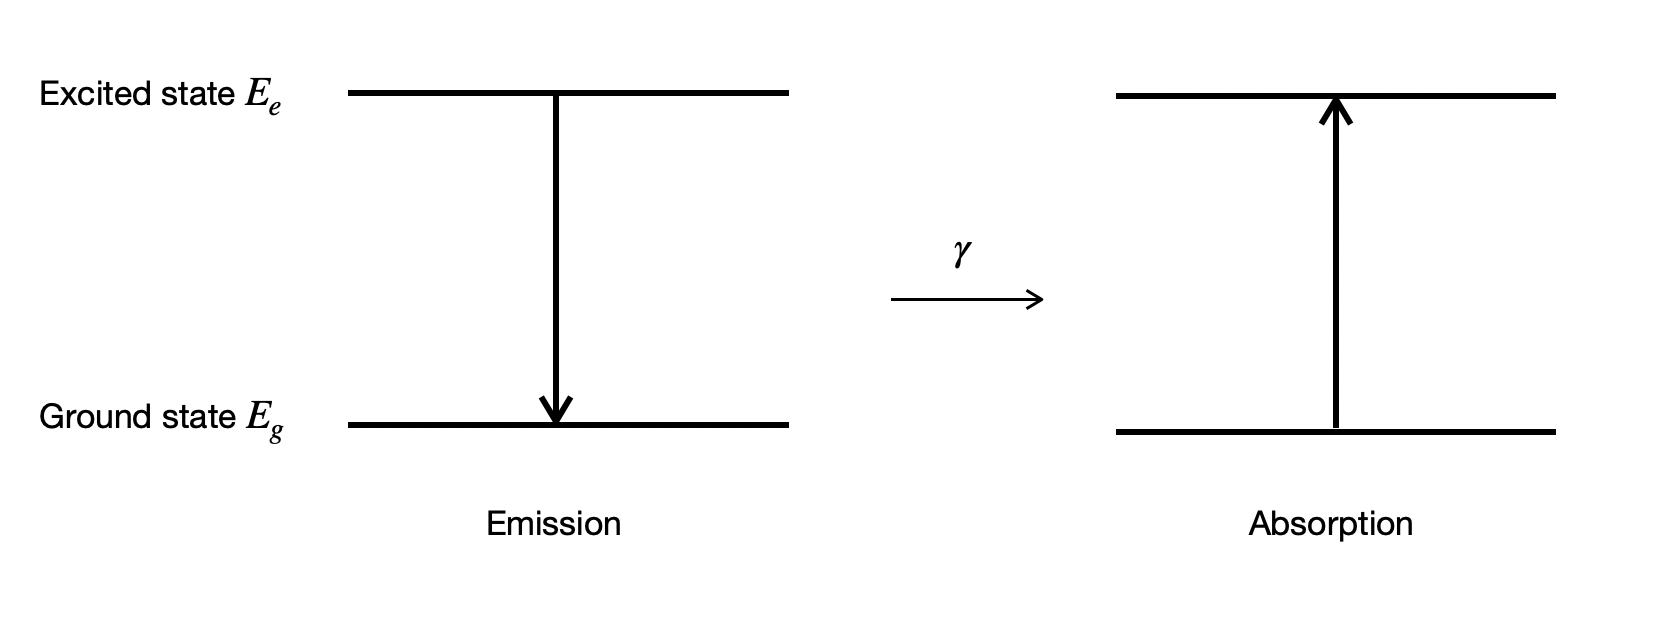
\includegraphics[width=0.8\textwidth]{moessbauer-effect}
    \caption{The recoilless emission and absorption of photon (M\"o{\ss}bauer effect).}
    \label{fig:moess}
\end{figure}

\subsection{Natural Linewidth}
The uncertainty in energy in the case of recoilless emission is limited by its natural linewidth. From the Heisenberg's uncertainty principle, we know that 

\begin{equation}
		\Delta E \Delta t = \hbar,
\end{equation}
where $\Delta E $ is the energy difference, $\Delta t$ is the time difference and $\hbar $ is the reduced Planck's constant. In our case, if we have a nuclear level with a mean lifetime of $\tau _{N}$, the energy uncertainty is given by

\begin{equation} \label{eqn:uncertainty}
		\Gamma = \hbar / \tau _{N}.	
\end{equation}

The frequency spectrum given by this emitted $\gamma$-ray is given by a Lorentz distribution, 

\begin{equation}
		I (\omega) = \frac{I_{0}}{1 + [2 \hbar (\omega - \omega_{0})/\Gamma]^2}
\end{equation}
where $I(\omega)$ is the intensity of the radiation at frequency $\omega$. The distribution (Fig. \ref{fig:lorentz}) is centered at $\omega_{0}$ and has a halfwidth of $\Gamma / \hbar $. For $^{57}$Fe used in this experiment, $\Gamma = 4.7 \times 10^{-9}$. 

\begin{figure}[htpb]
    \centering
    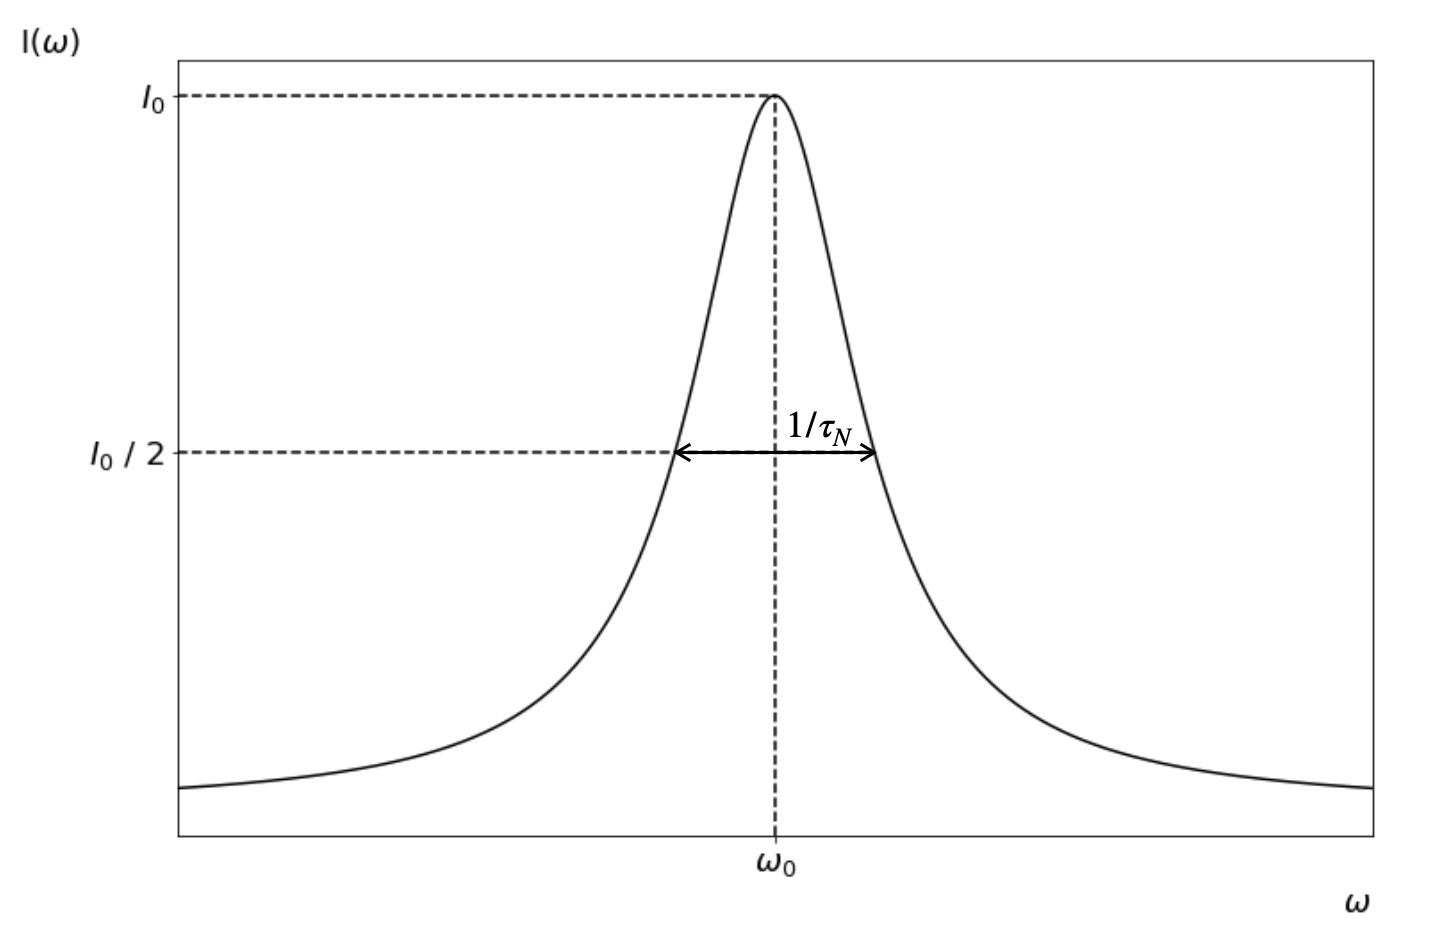
\includegraphics[width=0.8\textwidth]{lorentz}
    \caption{Intensity distribution of emitted $\gamma$-ray, centered at $\omega_{0}$ with a halfwidth of $1 / \tau _{N}$.}
    \label{fig:lorentz}
\end{figure}

\subsection{Recoil and Doppler Shift}

As discussed in Section \ref{sec:principles}, the recoil of the nucleus when emitting a $\gamma$-ray leads to a reduced energy. This can be written as

\begin{equation}
		E_{\mathrm{before}} = E_{e} + \frac{p^2}{2M},
\end{equation}
where, $p$ is the momentum and $M$ is the mass of the nucleus. Energy after the emission can be written as

\begin{equation}
		E_{\mathrm{after}} = E_{g} + \frac{(p - \hbar k)^2}{2M},
\end{equation}
where $\hbar k$ is the momentum of the emitted $\gamma$-ray. The energy difference is 

\begin{equation}
		E_{\mathrm{before}} - E_{\mathrm{after}} \equiv \hbar \omega = \hbar \omega_{0} + \hbar (k \cdot v) - \frac{\hbar ^2 k^2}{2M},
\end{equation}
where the term $\hbar (k \cdot v)$ is the Doppler effect, which is responsible for shift and broadening of the spectra. At room temperature, the Doppler shift for $^{57}$Fe is $\propto 10^{-2}$. The recoil energy $\hbar ^2 k^2 / 2M$ is $2 \times 10^{-3}$ eV, both of which are orders of magnitude greater than the natural width. The absorption and emission frequency spectrum is shown in Fig. \ref{fig:doppler}.

\begin{figure}[htpb]
    \centering
    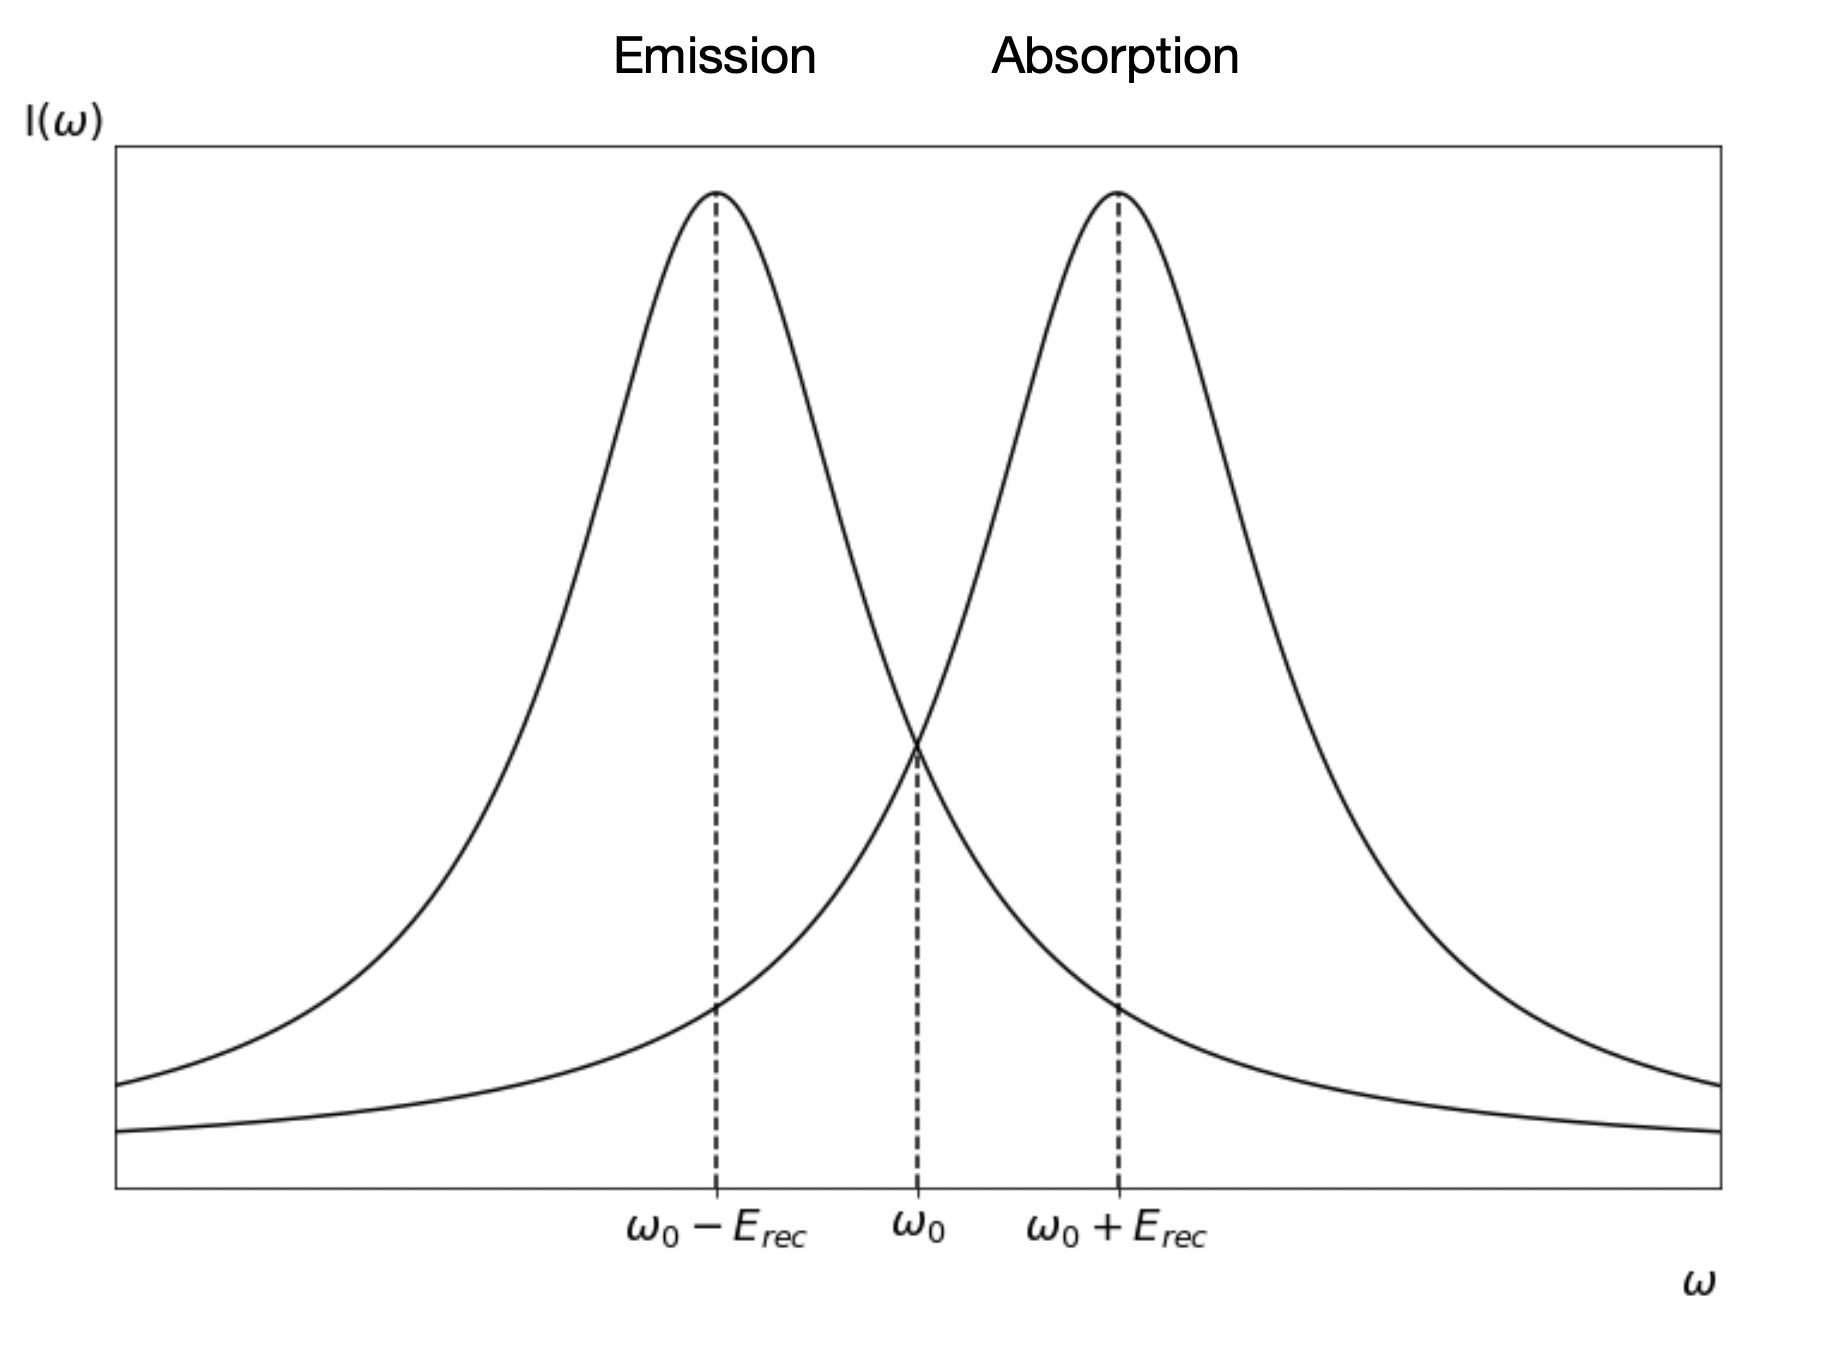
\includegraphics[width=0.8\textwidth]{doppler}
    \caption{Emission and absorption spectrum of a monoatomic gas in thermal equilibrium. Both the spectra are shifted by the recoil energy and have been broadened due to Maxwell velocity distribution.}
    \label{fig:doppler}
\end{figure}


\subsection{Debye-Waller Factor}
In a typical tightly bound solid, the energy required to displace an atom from its position is 20 eV. Since the recoil energy of the $\gamma$-ray is of the order $10^{-3}$ eV, there are two possibilities that can occur. One, since the atom cannot be displaced, it is set in a vibrational motion. Or second, if the vibrational motion is not altered by the emission, the recoil energy is absorbed by the entire solid. In a typical solid, the mass of the entire crystal is $10^{20}$ times more than the mass of the atom and hence the recoil energy is negligible. In this case, we get an unshifted, unbroadened, emission (M\"o{\ss}bauer) line. 

The Debye-Waller factor ($f(T)$) is defined is the ratio of the unshifted $\gamma$-ray emission to the total number of emissions. This ratio is dependent on temperature and is the highest at $T = 0 \si{\kelvin}$. But even at absolute zero, $f < 1$. This is because of zero-point energy. 

In order to understand the M\"o{\ss}bauer effect better, one needs to understand the Debye-Waller factor. Because this factor shows us why the M\"o{\ss}bauer fraction is large. Since the quantum mechanical derivation is a bit too complicated, we look at the semi-classical approach to gain an intuition behind the Debye-Waller factor.

\subsubsection{The Semiclassical Approach of the Debye-Waller Factor}
Let us consider a nucleus, continuously emitting an electromagnetic wave of frequency $\omega_{0} = E_{\gamma}/\hbar $ and oscillating around an equilibrium point. Considering only one vibration frequency $\Omega$, which corresponds to the Einstein model of the oscillations. The electric field of the emitted radiation is given by

\begin{equation} \label{eqn:emission}
		E(t) = E_{0} \exp\left(- i [\omega_{0} t + k x(t) ] \right),
\end{equation}
where $x(t) = a \sin (\Omega t)$, $a$ is the amplitude of the oscillation. Decomposition of this relation in Eqn. \ref{eqn:emission} shows that, the effect of vibration of the atom reduces the intensity of the central line by a factor of ($1 - k^2 a^2 / 4$) and also produces sidebands with frequencies $\omega_{0} \pm \Omega$, $\omega_{0} \pm 2 \Omega$, .... 

If we sum up these contributions to the intensity from sidebands to the unshifted line, we get

\begin{equation}
		A(\omega_{0}) = 1 - \frac{k^2 a^2}{4} + ... = \mathcal{J}_{0} (ka),
\end{equation}
where $\mathcal{J}_{0} (ka)$ is the Bessel function of zero order. The Debye-Waller factor is given by the absolute square of this quantity. 

So far we have considered only a single oscillation mode. When we consider several normal modes (phonons), in which each frequency produces its own sidebands, we need to take the product of all of them (Eqn. \ref{eqn:product}). 

\begin{equation} \label{eqn:product}
		f = \prod \mathcal{J}_{0}^2(ka_{n}) \approx \prod \left( 1 - \frac{k^2 a^2}{4}\right)^2 \approx \exp \left(- k^2 < x^2 > \right),   
\end{equation}
where $< x^2 > = \sum_{}^{} a_{n}^2 / 2$ is the average square displacement. For an isotropic, 3-dimensional oscillator, 

\begin{equation}
		f = \exp \left( - \frac{k^2 < u^2 >}{3} \right),
\end{equation}
where $< u^2 > = 3 < x^2 >$, the average square displacement. In quantum mechanics, this $< u^2 >$ becomes the expectation value.

Going back to the Einstein model, where only single vibration frequency $\Omega $ is considered, we can derive the temperature dependence for the Debye-Waller factor. The harmonic energy with $n$ excited quanta is taken, the occupation probability is calculated and we find that the Bose-Einstein distribution function is obtained. Using this result, we then generalize for a phonon distribution function $Z(\Omega )$ and calculate the dependence for 3-dimensions. The result we obtain is

\begin{equation}
		f(T) = \exp \left( - \frac{\hbar k^2}{6 M N } \int\limits_{0}^{\infty} \frac{Z(\Omega )}{\Omega } \left[ 1 + \frac{2}{\exp(\hbar \Omega / k_{b} T) - 1 } \right] d \Omega \right),
\end{equation}
where $N$ is the number of molecules in the solid. 

The following important conclusions can be deduced: 
\begin{enumerate}
		\item By measuring the Debye-Waller factor, one can obtain the phonon frequency spectrum.
		\item The Debye-Waller factor decreases with increase in the recoil energy.
		\item Large M\"o{\ss}bauer effect can be observed at low temperatures, which is because of the fact that the Debye-Waller factor is maximum at absolute zero. Hence, low temperatures are favorable for measurement.
\end{enumerate}

\section{M\"o{\ss}bauer Source}

There are several requirements for a M\"o{\ss}bauer source. These are: 

\begin{enumerate}
		\item The $\gamma$-ray transition must go to the ground state, since for a stable isotope, absorption can only take place from the ground state.
		\item The Debye-Waller factor must not be too small. In order to achieve that, we must have low temperatures, low $\gamma$-ray energy, high Debye temperature and high atomic mass.
		\item The lifetime should not be too short, otherwise due to Eqn. \ref{eqn:uncertainty}, we will have a poor energy resolution.
		\item The source should be practical (easy to obtain, handle and so on).
\end{enumerate}

There are several possible sources for studying the M\"o{\ss}bauer effect, many of these are discussed in detail in \cite{Schatz1996}. In this experiment, we used isotope $^{57}$Co as the source. The decay scheme is shown in Fig. \ref{fig:decay}.

\begin{figure}[htpb]
    \centering
    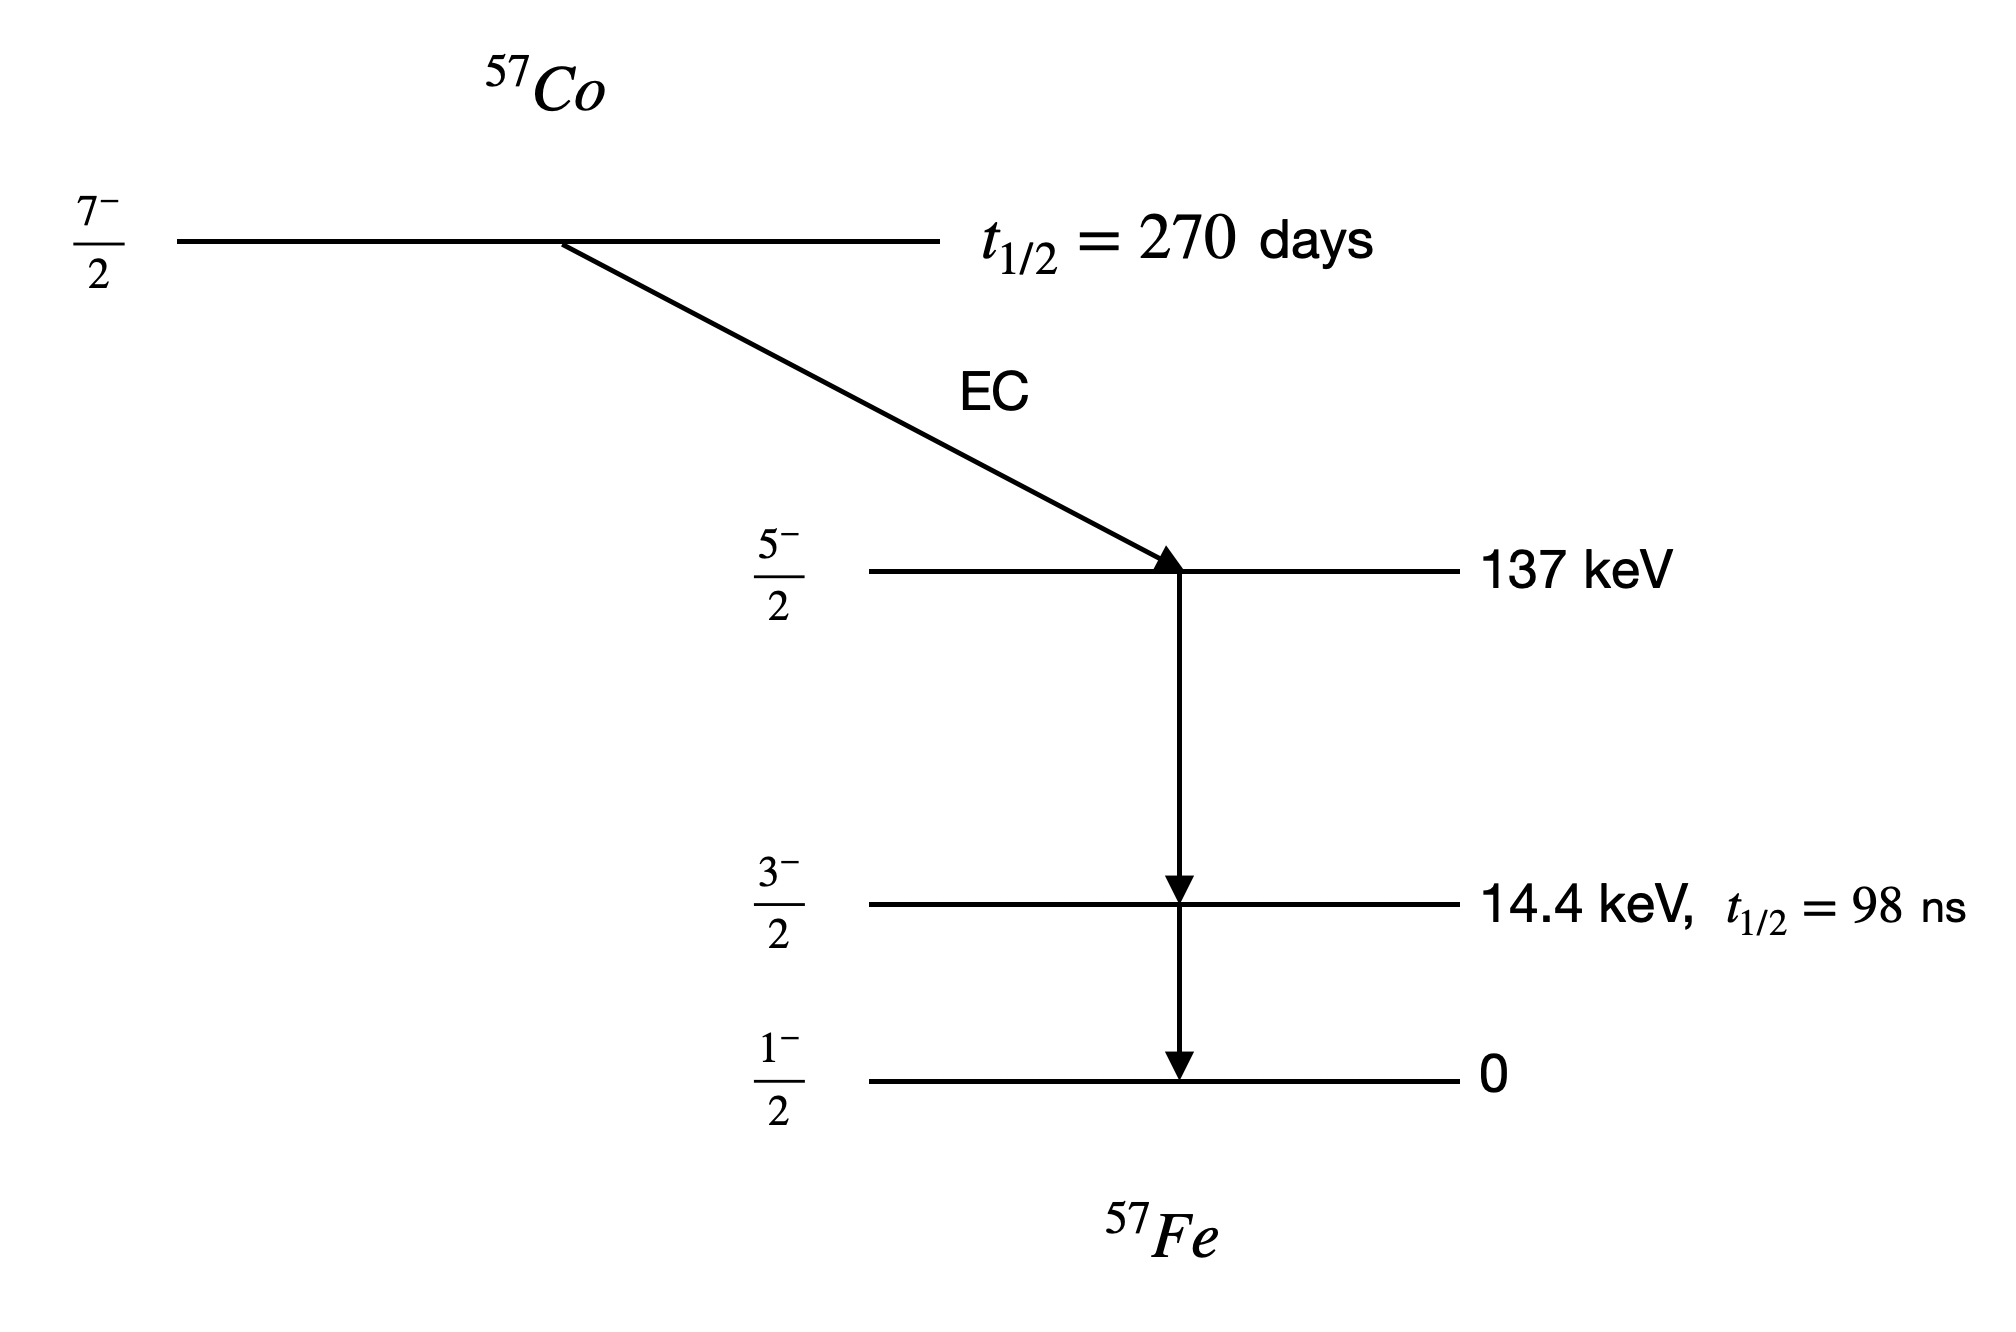
\includegraphics[width=0.8\textwidth]{source}
    \caption{Decay scheme of $^{57}$Co. The decay occurs largely (99.8\%) due to Electron Capture (EC). The nuclear moments of M\"o{\ss}bauer level (I = 3/2) and ground level (I = 1/2) are shown here.}
    \label{fig:decay}
\end{figure}	

The M\"o{\ss}bauer source $^{57}$Co - $^{57}$Fe is an ideal choice because the parent isotope, $^{57}$Co has long halflife (270 days), which enables one to perform several experiments with the same source. The lifetime of the M\"o{\ss}bauer level is sufficiently long, giving us a good energy resolution. Lastly, the energy level of 14.4 keV is small enough to allow for the conduction of experiment at room temperature. 

\section{Isomer Shift}

\section{Electric Quadrupole Interaction}

\section{Magnetic Dipole Interaction}

\section{M\"o{\ss}bauer Apparatus and Setup}


\chapter{Experimental Set-Up}

To measure the Moessbauer spectrum, we placed a Co-57 radioactive source onto a table with a moving absorber 
that has a maximum displacement of $\SI[]{25.1 \pm 0.2}[]{\milli\metre}$.  A photodetector is placed 
behind the absorber that detects the number of photons that are not absorbed via this process. The speed of the 
absorber is controlled by a motor that swings the absorber at a fixed velocity. See Fig. \ref{apparatus_source}
for the Moessbauer source apparatus. \par 

\begin{figure*}[htb!]
	\centering
	\includegraphics[width=0.7\columnwidth]{source_image.png}

	\caption{The set-up of the Moessbauer source. \textit{Left}: The Co-57 source. \textit{Middle}: 
	The moving absorber. \textit{Right}: The photodetector which is connected to the detector apparatus.
	}
	\label{fig:apparatus_source}
\end{figure*}

The photodetector is then connected to a single channel analyzer (SCA), which determines the number of counts detected
in a given time range and maximal and minimal width to observe the counts. The SCA has 2 main parameters that should be modified:
the Upper Level Discrimator (ULD) and the Lower Level Discrimator (LLD), which controls the binsize and the lower limit for 
photodetection respectively. The modes of the ULD can be set to measure with a higher resolution by detecting counts with 
10 $\%$ of the binsize. The SCA was then connected to a display in which the number of counts obtained in a specific time 
interval was shown. 
The photodetecting apparatus consisted of two such setups to consider for measurements with positive and negative velocity 
of the absorber as the offset voltage between the two can allow the measurements in the LR and RL direction to differ.
A separate run counter that tracks the number of turns that the absorber had is also contained in the apparatus. A timer 
that controls the time interval of measurement is also placed which is used for the calibration process. The set-up is 
constructed in a way such that the count and time measurements terminate only after the absorber had performed a full turn. 
See Fig. \ref{fig:apparatus_raw} for the apparatus used for the photodetection as well as the schematic of the apparatus. \par 

\begin{figure*}[htb!]
	\centering
	\subfloat[]{{\includegraphics[width=0.45\columnwidth]{apparatus_image.png}}}
	\quad
	\centering
	\subfloat[]{{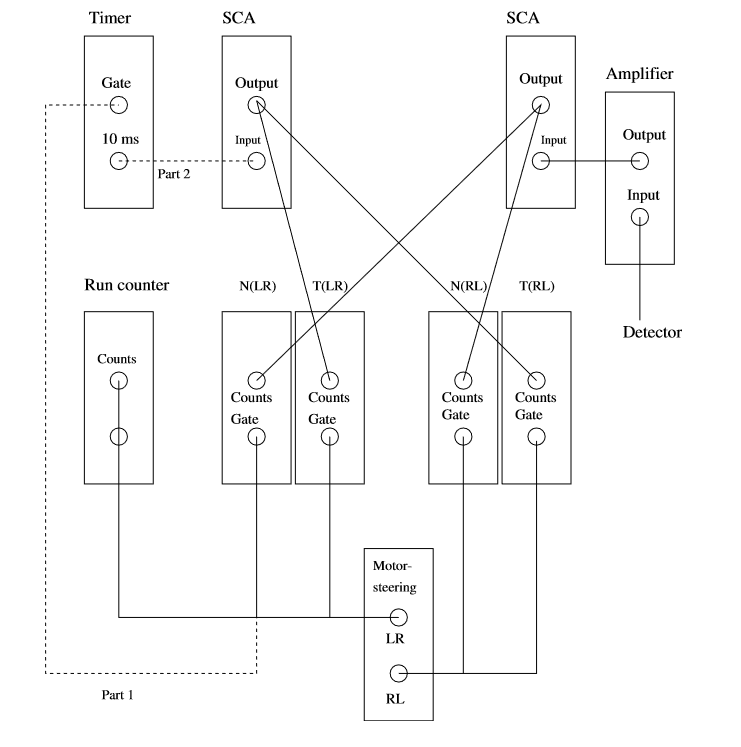
\includegraphics[width=0.45\columnwidth]{apparatus_schematic.png}}}
	\caption{(a) The photodetector apparatus used in this experiment. (b) The schematic of the apparatus. Obtained from 
			Ref. \cite{k2212016}.}
	\label{fig:apparatus_raw}
\end{figure*}

% \section{Procedure}

% \subsection{Calibration of SCA}
\chapter{Calibration} \label{sec:calibration}

Before we took any measurements, we determined the optimal values for the LLD in order to ensure that we are 
detecting counts from the 14.4 keV transition. In order to do so, we modified the LLD from 0 to 4 and determined the number 
of counts obtained at each value for a fixed time interval for $T = \SI{10}{\second}$. Once the data was obtained, 
we plotted the number of detected photons $N$ against the LLD values and compared our results to the Fe-57 $\gamma$-spectrum as seen in Fig. \hl{add reference here}.
This allowed us to identify the range in which we should set the ULD and LLD values when performing the Moessbauer measurements. 
 Fig. \ref{fig:calibration_plot} shows the obtained spectrum from our experiment. See the Appendix section for the full data obtained from this 
 section. The uncertainty for the counts were taken to be purely statistical such that $\delta N = \sqrt{N}$, and the uncertainty 
 of the time interval measurement was taken to be $\delta T = \pm \SI{0.003}{\second}$. \par

\begin{figure*}[htb!]
	\centering
	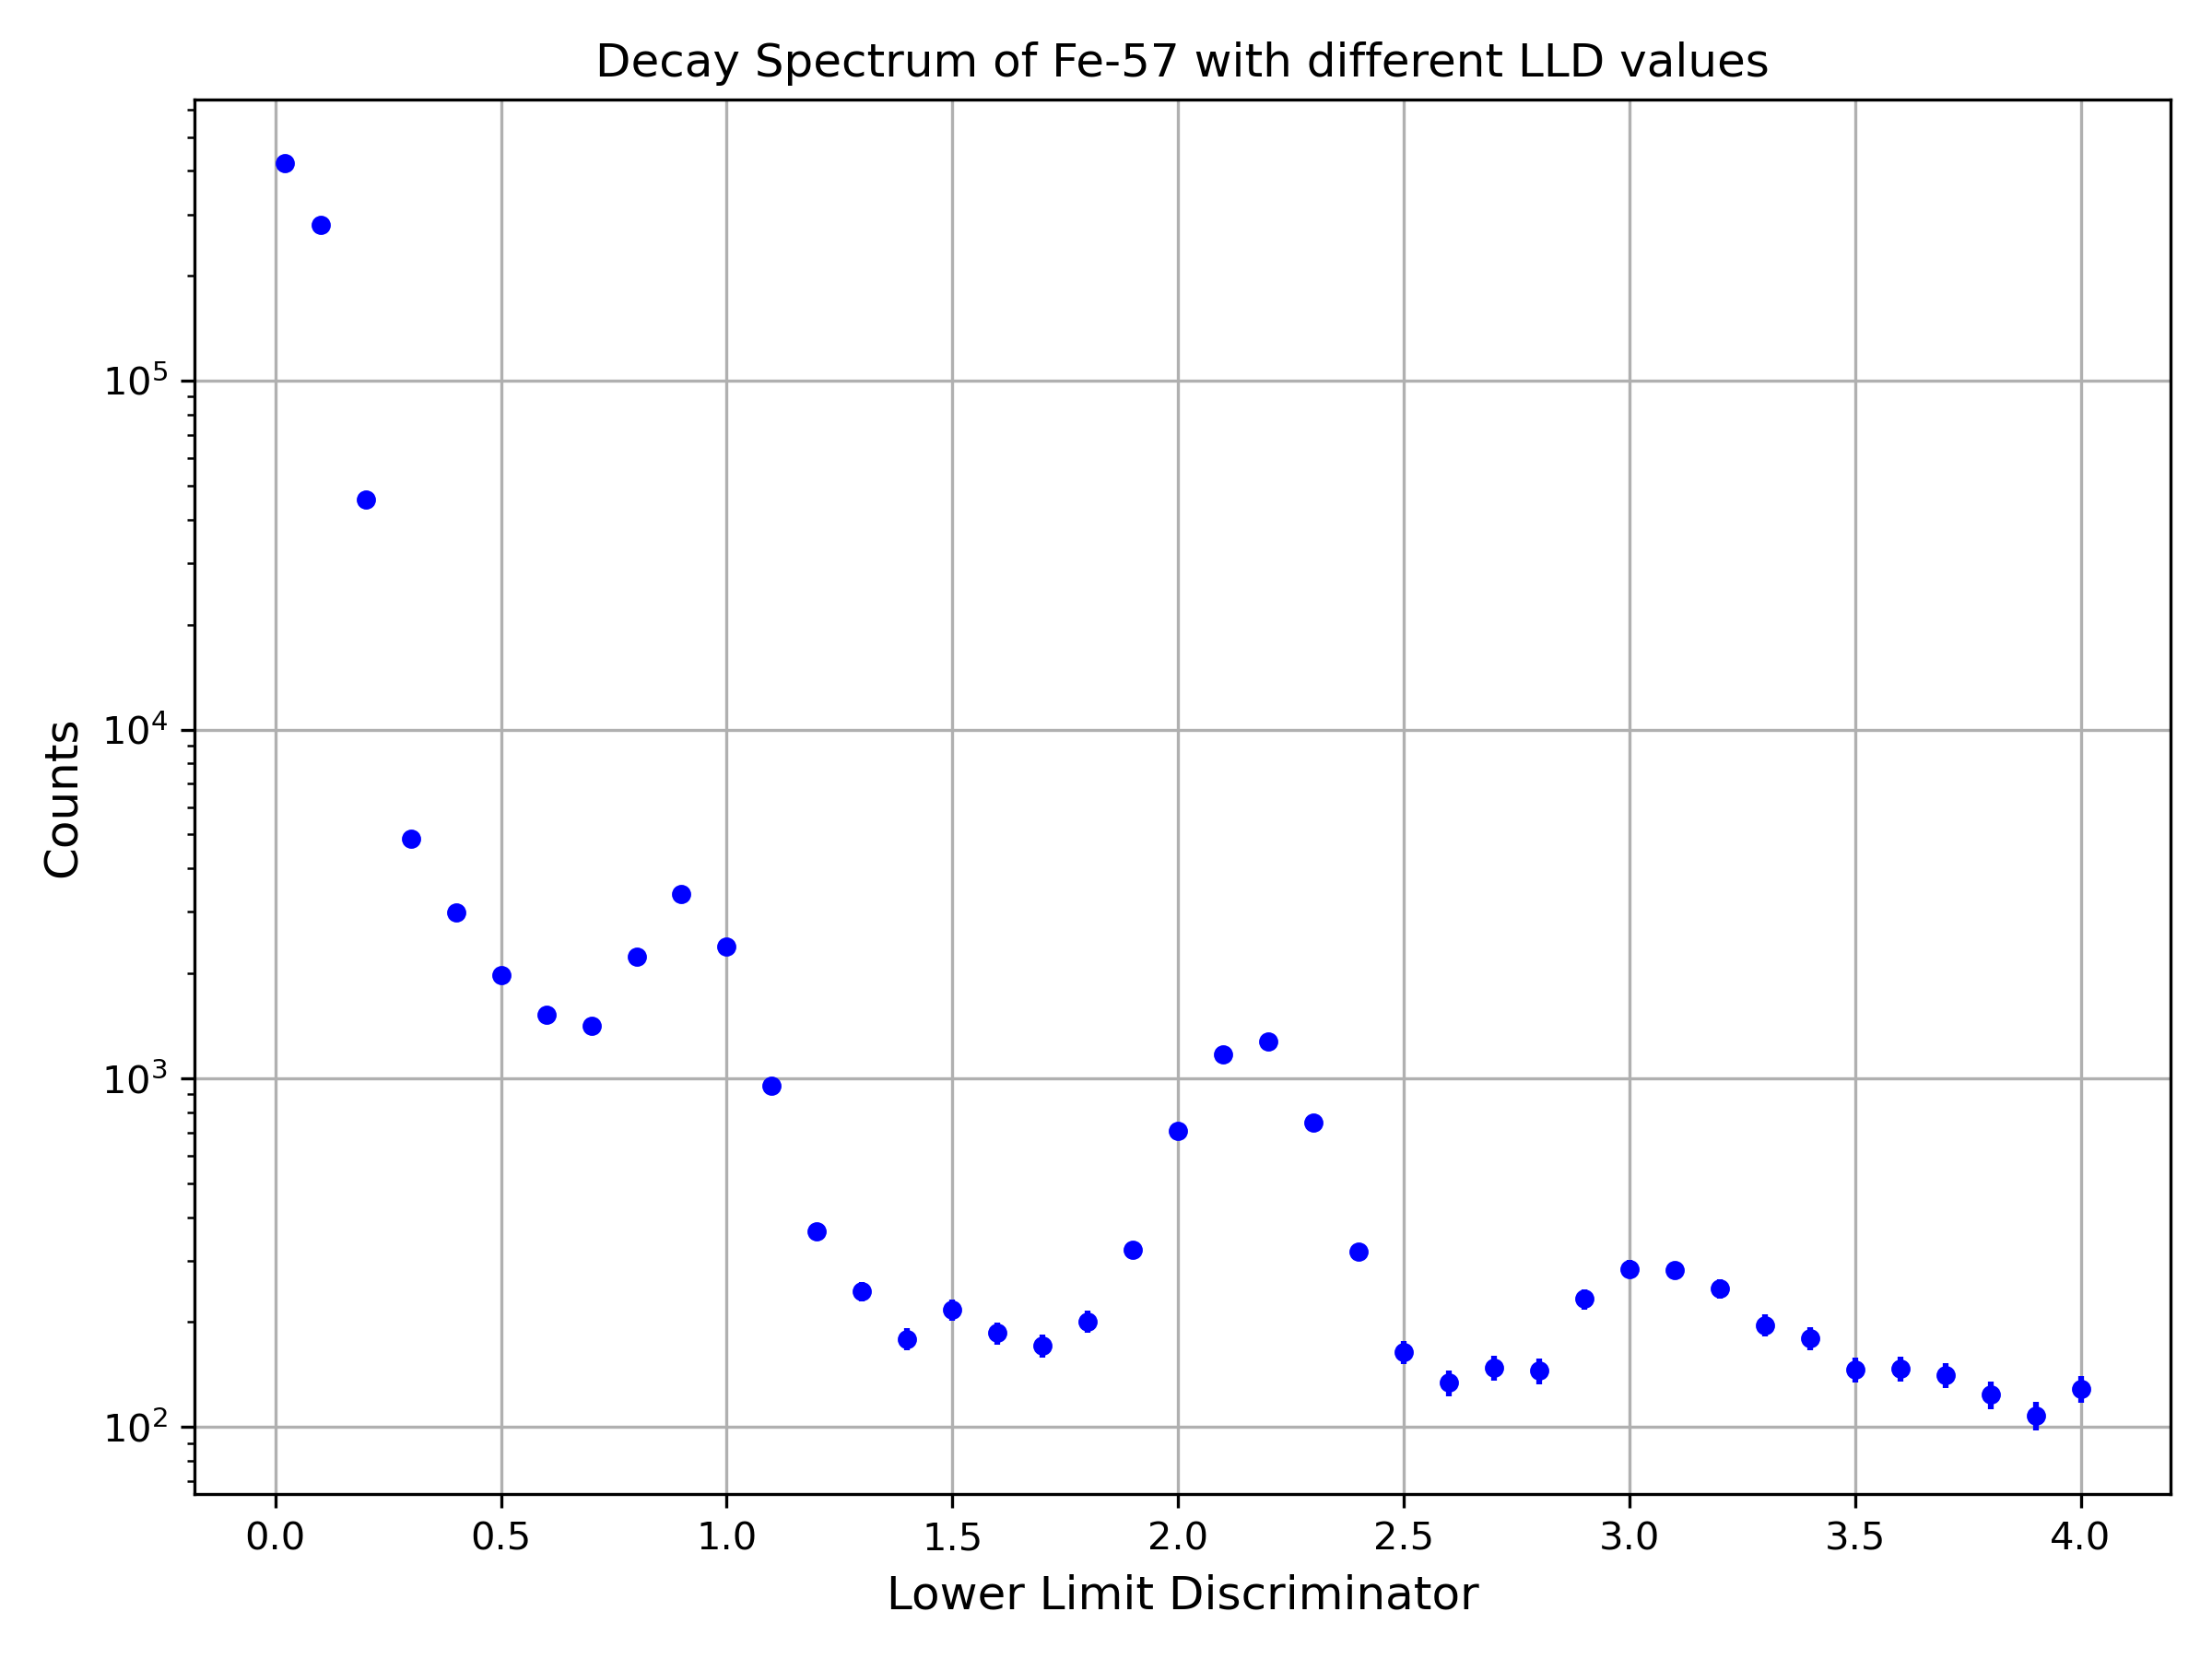
\includegraphics[width=0.7\columnwidth]{calib_plot.png}
	\caption{The pulse height spectrum for Fe-57 decay observed in the experiment. The number of counts are shown for varying 
	LLD values.}
	\label{fig:calibration_plot}
\end{figure*}

By comparison to expected results, we identified the 14.4 keV transition line as the third peak on Fig. \ref{fig:calibration_plot}. 
The ULD and LLD values that were used to perform the Moessbauer measurement was then set to be 1.8 and 2.6 respectively. \par 

% add something about how we used fit to get the true values for the LLD values (if we do)?

% \chapter{Results and Discussion}

\chapter{Moessbauer Spectrum}

\section{Procedure and Results}

To observe the Moessbauer spectrum, we first set the ULD and LLD to 1.8 and 2.6 respectively as obtained from Chapter \ref{sec:calibration}. 
Once a certain motor speed has been set, we ran both LR and RL single channel analyzer for a set number of turns, ranging from 4 to 10
turns. We then recorded the obtained number of counts and duration for both LR and RL analyzers. This was repeated until we obtained 
enough points to more accurately construct the Moessbauer peaks. This was verified by using the built-in plotting tool in Excel where we 
displayed the plot between the count rate $R = N / T$ against the motor speed. We took a total of 60 measurements in this experiment, ranging for 
motor speeds from 0 to 2.5. Fig. \ref{fig:moess_raw} shows the raw data obtained from both analyzers. See Appendix (Chapter \ref{sec:Appendix}) for the raw data table obtained from both analyzers. \par 

\begin{figure*}[htb!]
	\centering
	\subfloat[]{{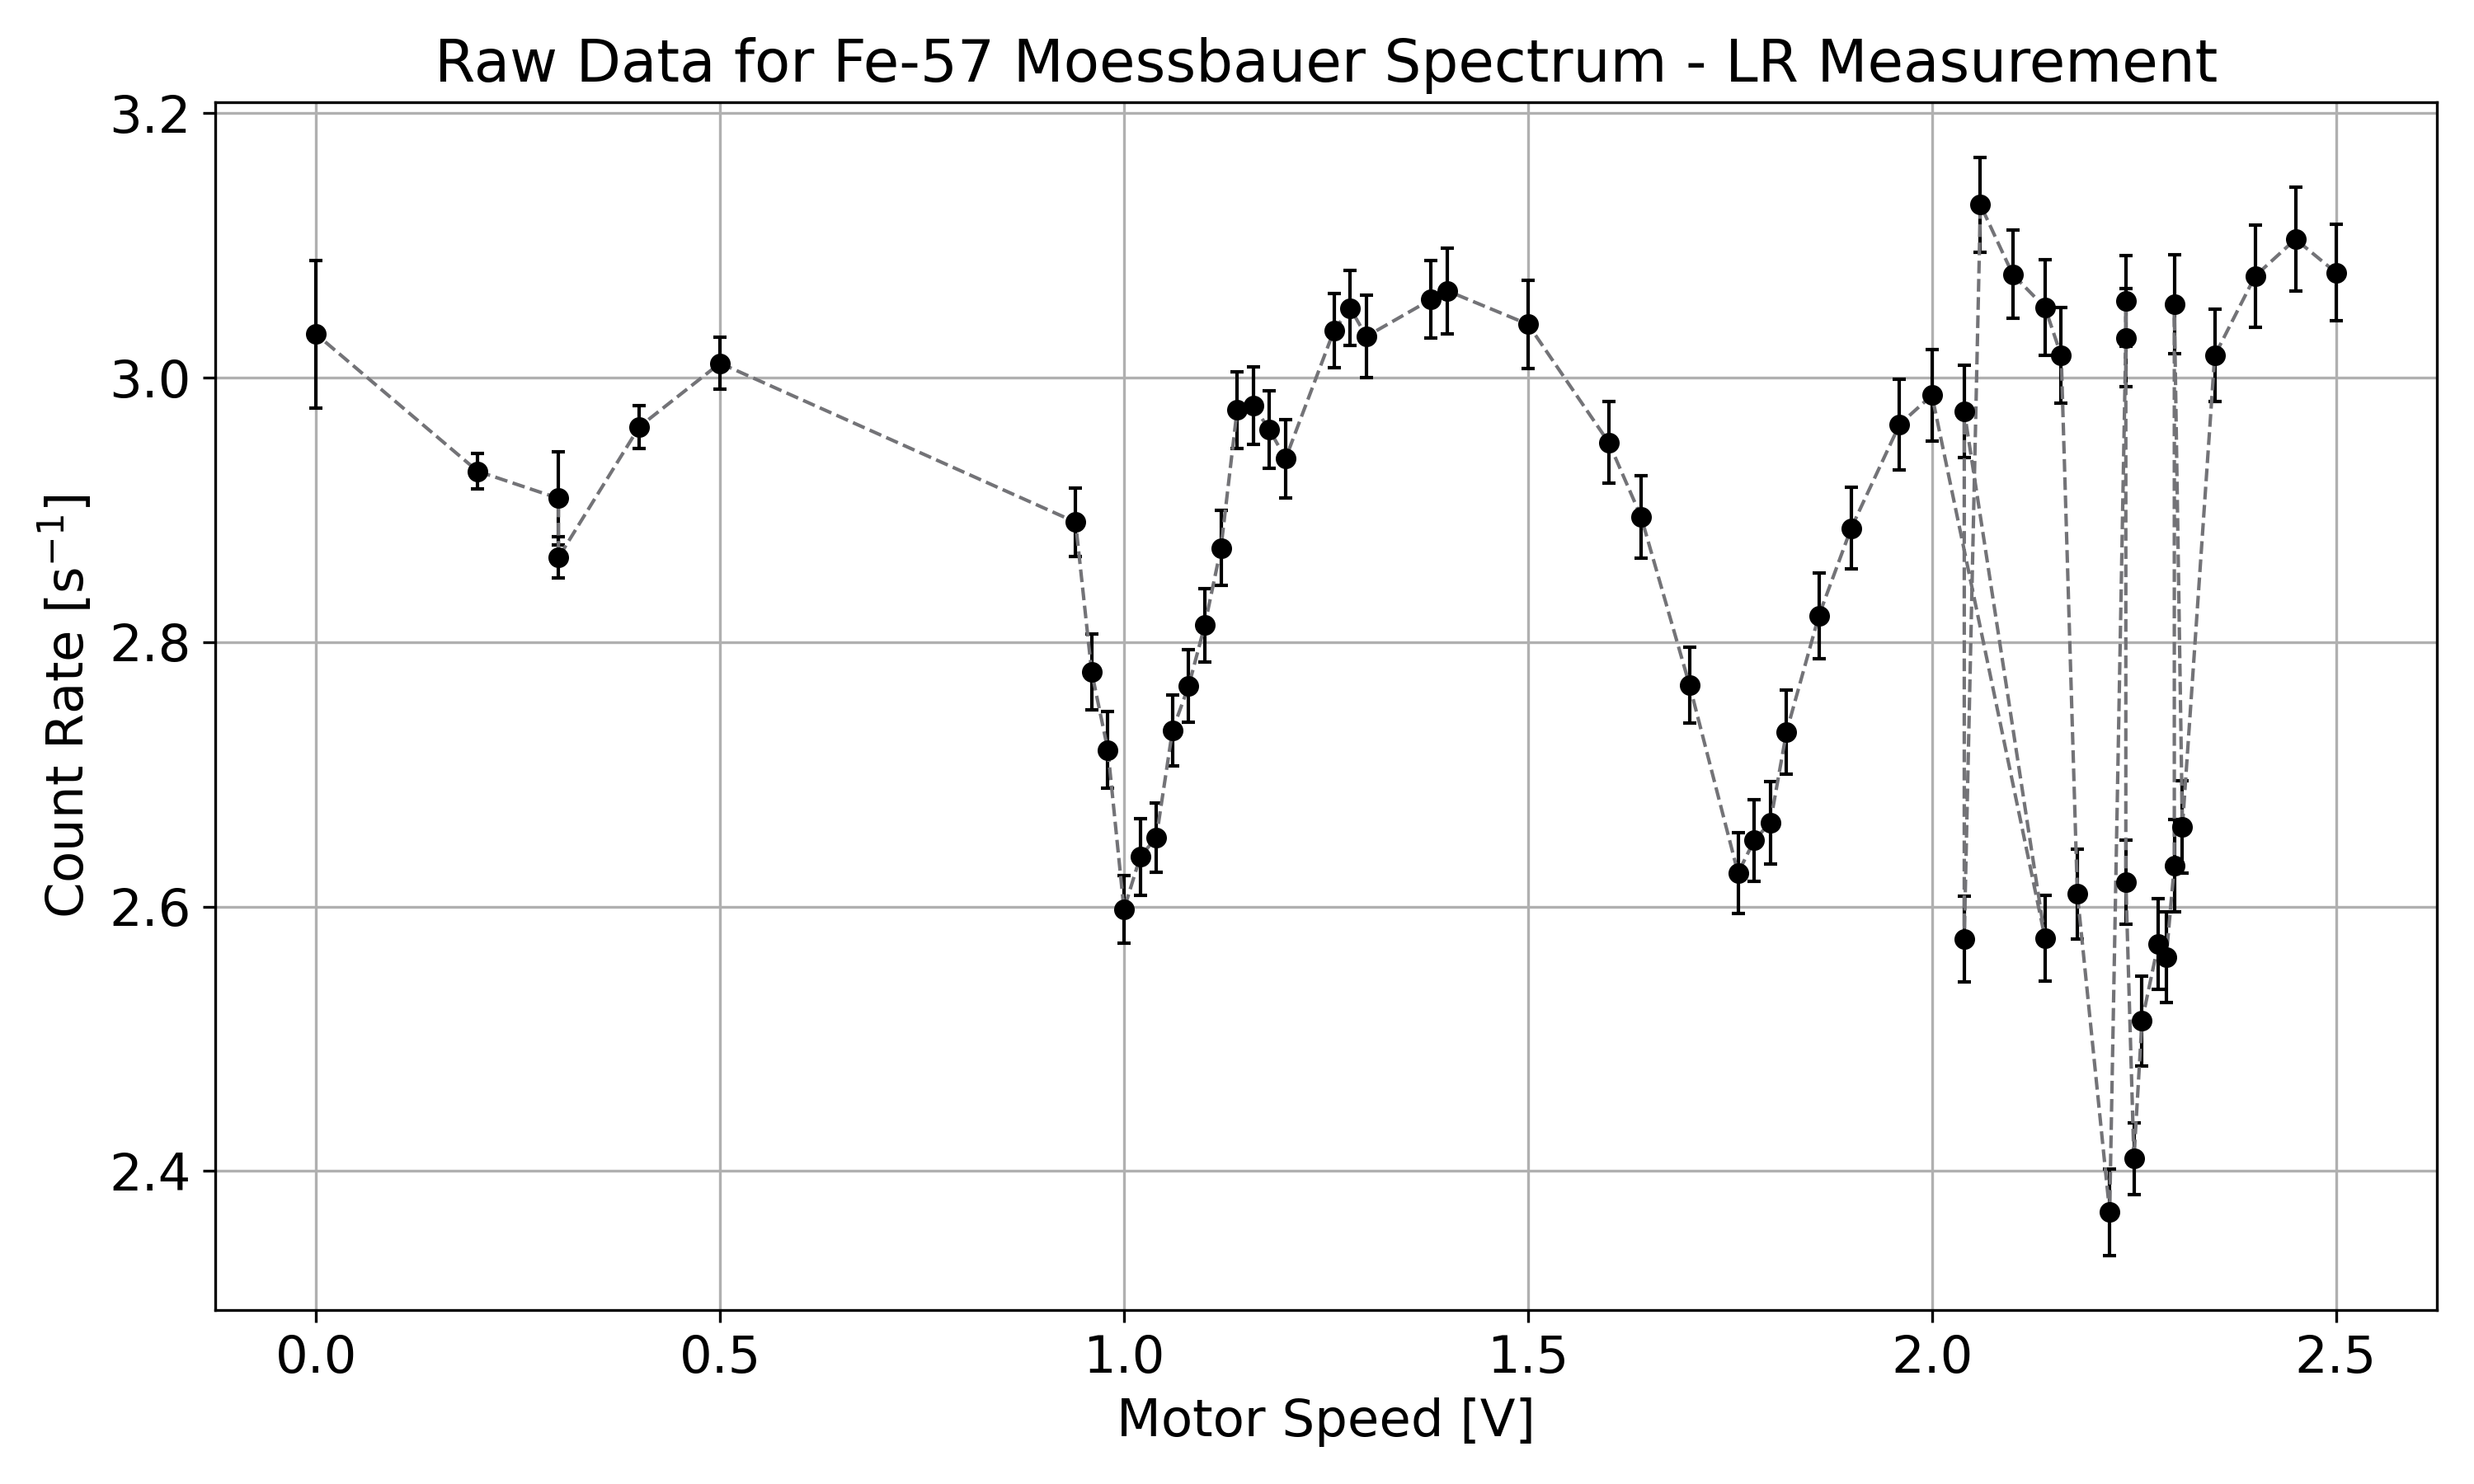
\includegraphics[width=0.45\columnwidth]{raw_moess_LR.png}}}
	\quad
	\centering
	\subfloat[]{{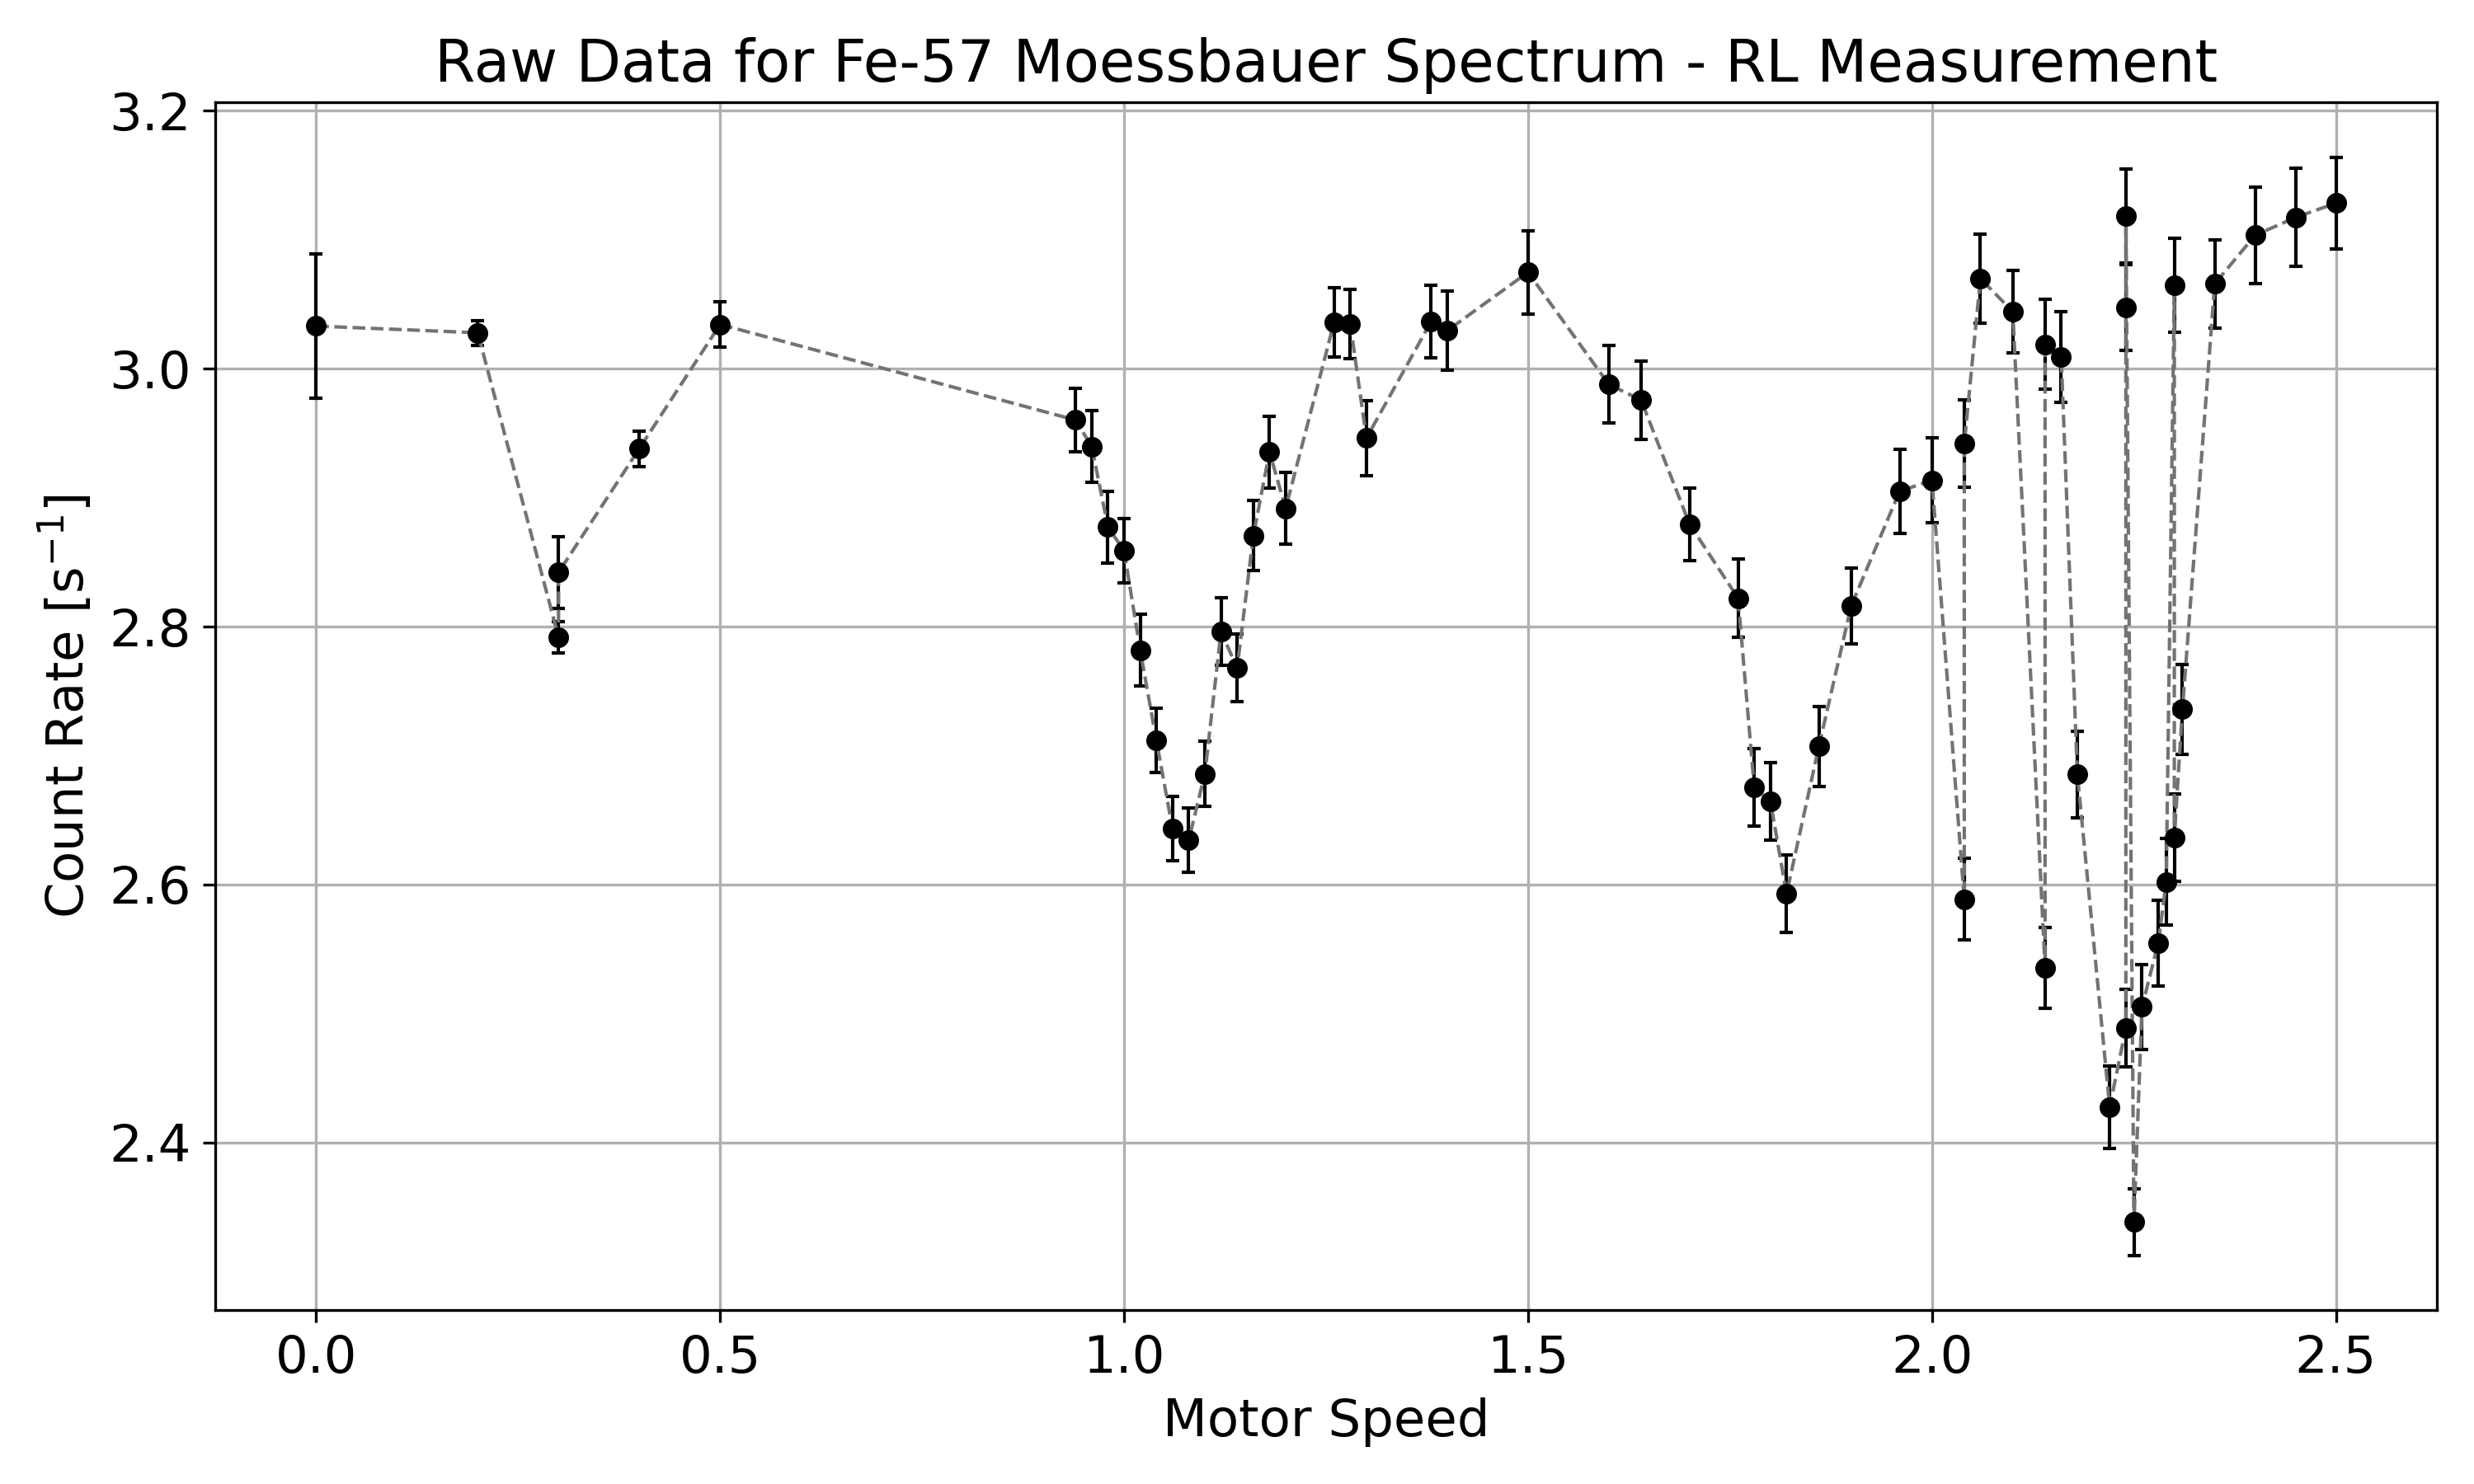
\includegraphics[width=0.45\columnwidth]{raw_moess_RL.png}}}
	\caption{The Raw Spectrum obtained from the Moessbauer measurement for the 14.4 keV transition for Fe-57 from the (a) LR and (b) RL 
	single channel analyzer. Several outliers can be observed.}
	\label{fig:moess_raw}
\end{figure*}


The uncertainty of the count rate was calculated using the standard Gaussian error propagation formula using $\delta N$, $\delta T$ 
as in Chapter \ref{sec:calibration}:
\begin{equation}
	\delta R = R \sqrt{\left(\frac{\delta N}{N}\right)^2 + \left(\frac{\delta T}{T}\right)^2} = R \sqrt{\left(\frac{\sqrt{N}}{N}\right)^2 + \left(\frac{\delta T}{T}\right)^2} .
\end{equation} \par 


To determine the peaks, we first filtered out the outliers from the data, then combined the LR and RL measurements to construct 
the full Moessbauer spectrum. We then performed a non-linear fit to the multi-Lorentzian distribution, i.e. the sum of Lorentzian
distributions, to determine the peak velocity $v_0$, peak amplitude $I_0$, and uncertainty $\Gamma_v$ for each observed peak. The 
offset $\delta_v$ from a full symmetric distribution was also determined through this fitting process. This was done using the Python package \texttt{lmfit} that utilizes the Levenberg-Marquardt method. Fig. \ref{fig:moess_spect} shows the full Moessbauer
spectrum with the obtained Lorentzian fit. Table \ref{tab:fit_params} shows the obtained fit parameters from the analysis for each peak.
The offset was determined to be $\delta_v = \SI{3.131 \pm 0.020}{\milli\meter\per\second} $. \par 


\begin{figure*}[htb!]
	\centering
	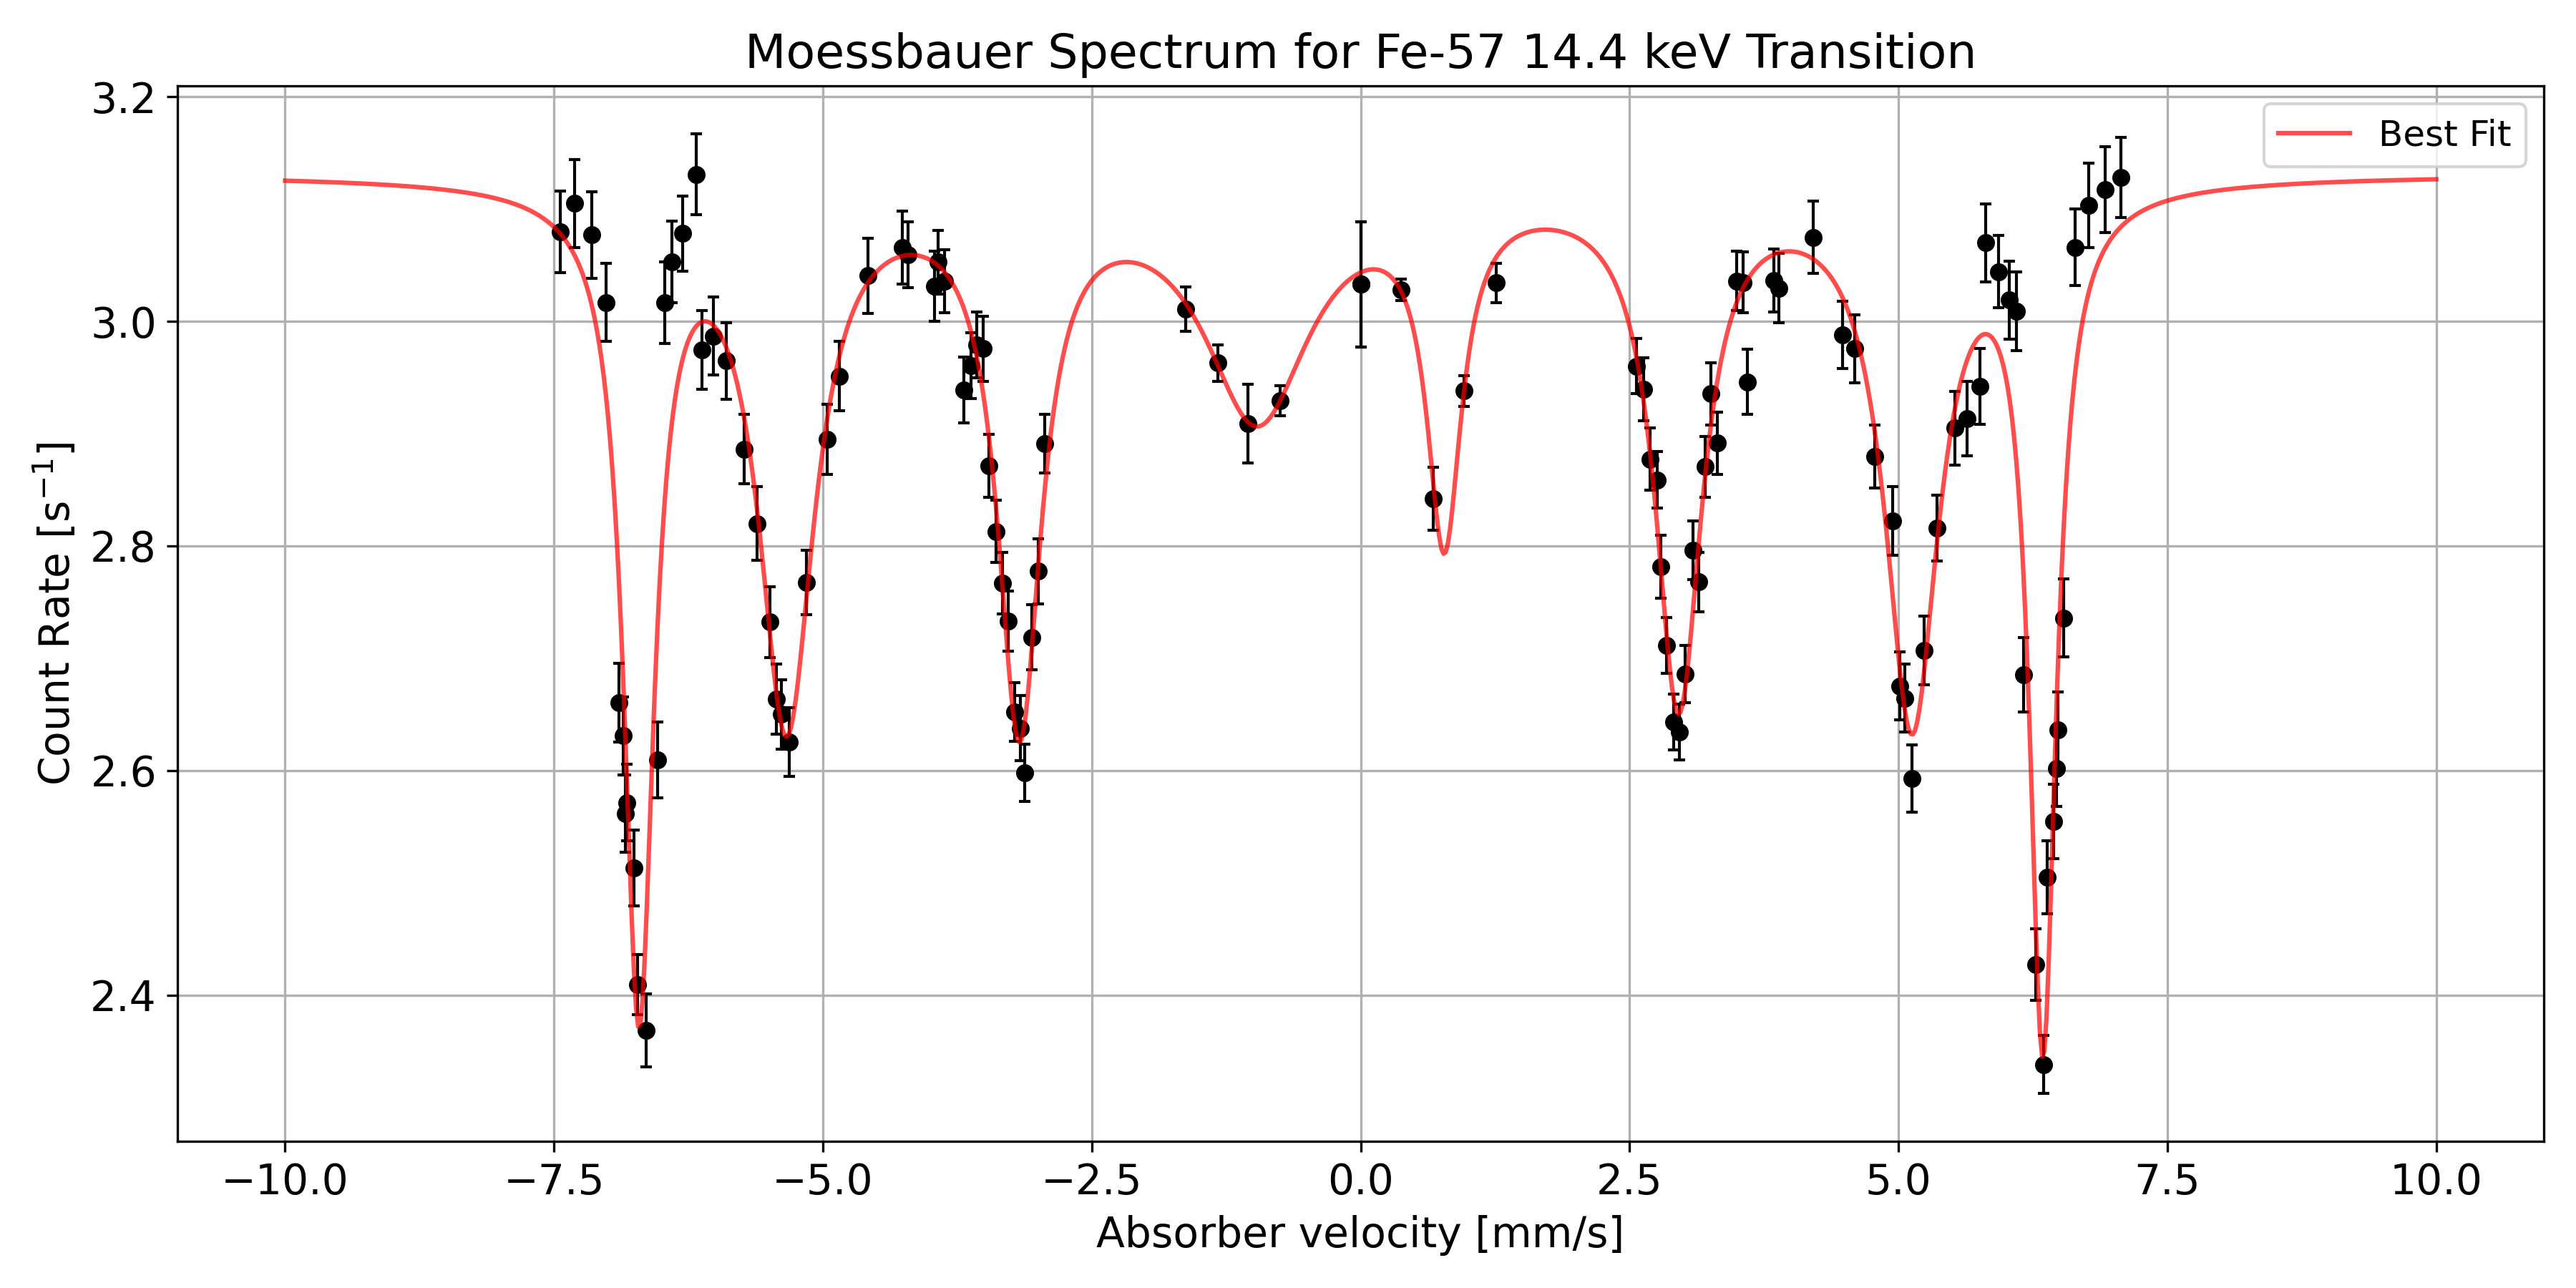
\includegraphics[width=0.8\columnwidth]{moess_spect.png}
	\caption{The observed Moessbauer spectrum for Fe-57 through the 14.4 keV transition for varying absorber velocities. The 
	non-linear Lorentzian fit is also shown.}
	\label{fig:moess_spect}
\end{figure*}

\begin{table}[!ht]
    \centering
    \begin{tabular}{|c|c|c|c|c|}
    \hline
        Peak & $v_0$ [$\si[]{\milli\meter\per\second}$] & $I_0$  & $\Gamma_v$ [$\si[]{\milli\meter\per\second}$] & $\delta_v - I_0$\\ \hline
        1 &$ -6.710 \pm 0.010$ & $0.731 \pm 0.037$ & $ 0.346 \pm 0.033$ & $2.400 \pm 0.042$\\ \hline
        2 &$ -5.337 \pm 0.025 $ & $0.479 \pm 0.034$ & $ 0.630 \pm 0.090$ & $2.653 \pm 0.040$\\ \hline
        3 &$ -3.172 \pm 0.013 $ & $0.478 \pm 0.026$ & $ 0.496 \pm 0.053$ & $2.654 \pm 0.033$\\ \hline
        4 &$ -0.963 \pm 0.073 $ & $0.209 \pm 0.033$ & $ 1.21 \pm 0.50$ & $2.923 \pm 0.039$\\ \hline
        5 &$ 0.778 \pm 0.019 $ & $0.303\pm 0.067$ & $ 0.39\pm 0.12$ & $2.829 \pm 0.070$\\ \hline
        6 &$ 2.956\pm 0.012 $ & $0.461 \pm 0.024$ & $ 0.529 \pm 0.051$ & $2.670 \pm 0.031$\\ \hline
        7 &$ 5.125 \pm 0.023 $ & $0.477 \pm 0.033$ & $ 0.610 \pm 0.085$ & $2.654 \pm 0.039$\\ \hline
        8 &$ 6.3430 \pm 0.0091 $ & $0.754 \pm 0.034$ & $ 0.3042 \pm 0.027$ & $2.378 \pm 0.040$\\ \hline
    \end{tabular}
	\caption{Fit parameters $v_0$, $I_0$, and $\Gamma_v$ obtained for each peak. The peak values $\delta_v - I_0$ 
			as shown in Fig. \ref{fig:moess_spect} is also presented.
			 The peak is numbered from the left most peak to the rightmost peak.}
	\label{tab:fit_params}
\end{table}





\section{Discussion}


\chapter{Conclusion and Outlook}

\chapter{Acknowledgements}
We would like to take this moment and thank Dr. Barth, who was really helpful and patient with us. We were lucky to have him as our tutor. Next, we would like to thank...


\printbibliography

\chapter{Appendix} \label{sec:Appendix}

In the following section, we include all the data which was measured while performing the experiment.

\begin{table}[!ht]
    \centering
	\begin{tabular}{|c|c|c|c|}
    \hline
	Lower Limit Discriminator $\pm$ 0.01 & Count (N) & Time (s) $\pm$ 0.03 & Upper Level Discriminator ($\Delta$ E) (100\%) ($10^{-1}$)) \\ \hline
        0.02 & 420580 & 10 & 10 \\ \hline
        0.10 & 279704 & 10 & 10 \\ \hline
        0.20 & 45643 & 10 & 10 \\ \hline
        0.30 & 4853 & 10 & 10 \\ \hline
        0.4 & 2982 & 10 & 10 \\ \hline
        0.5 & 1981 & 10 & 10 \\ \hline
        0.6 & 1522 & 10 & 10 \\ \hline
        0.7 & 1412 & 10 & 10 \\ \hline
        0.8 & 2227 & 10 & 10 \\ \hline
        0.9 & 3368 & 10 & 10 \\ \hline
        1 & 2386 & 10 & 10 \\ \hline
        1.1 & 952 & 10 & 10 \\ \hline
        1.2 & 365 & 10 & 10 \\ \hline
        1.3 & 245 & 10 & 10 \\ \hline
        1.4 & 179 & 10 & 10 \\ \hline
        1.5 & 217 & 10 & 10 \\ \hline
        1.6 & 186 & 10 & 10 \\ \hline
        1.7 & 171 & 10 & 10 \\ \hline
        1.8 & 201 & 10 & 10 \\ \hline
        1.9 & 322 & 10 & 10 \\ \hline
        2 & 705 & 10 & 10 \\ \hline
        2.1 & 1169 & 10 & 10 \\ \hline
        2.2 & 1275 & 10 & 10 \\ \hline
        2.3 & 745 & 10 & 10 \\ \hline
        2.4 & 319 & 10 & 10 \\ \hline
        2.5 & 164 & 10 & 10 \\ \hline
        2.6 & 134 & 10 & 10 \\ \hline
        2.7 & 148 & 10 & 10 \\ \hline
        2.8 & 145 & 10 & 10 \\ \hline
        2.9 & 233 & 10 & 10 \\ \hline
        3 & 284 & 10 & 10 \\ \hline
        3.1 & 282 & 10 & 10 \\ \hline
        3.2 & 249 & 10 & 10 \\ \hline
        3.3 & 196 & 10 & 10 \\ \hline
        3.4 & 180 & 10 & 10 \\ \hline
        3.5 & 146 & 10 & 10 \\ \hline
        3.6 & 147 & 10 & 10 \\ \hline
        3.7 & 141 & 10 & 10 \\ \hline
        3.8 & 124 & 10 & 10 \\ \hline
        3.9 & 108 & 10 & 10 \\ \hline
        4 & 129 & 10 & 10 \\ \hline
    \end{tabular}
    \caption{Calibration of the single channel analyzer.}
    \label{calibration}
\end{table}


\hl{Verify the unit of motor speed.}
\begin{table}[!ht]
    \centering
    \begin{tabular}{|c|c|c|c|c|c|}
    \hline
        Velocity (mm/s) & Motor speed (V) & Count (N) (RL) & Time (ms) (RL) & Number of turns & Count/s (N/s) \\ \hline
        0 & 0 & 3030 & 999 & 0 & 3.03303303303303 \\ \hline
        0.375400077772128 & 0.2 & 101223 & 33431 & 5 & 3.02781849181897 \\ \hline
        0.674368619022031 & 0.3 & 10578 & 3722 & 1 & 2.8420204191295 \\ \hline
        0.959174574867843 & 0.4 & 46130 & 15701 & 6 & 2.9380294248774 \\ \hline
        1.25827150591538 & 0.5 & 30264 & 9974 & 5 & 3.03428915179467 \\ \hline
        2.56488861639076 & 0.94 & 14484 & 4893 & 5 & 2.96014714898835 \\ \hline
        2.62964903090623 & 0.96 & 11223 & 3818 & 4 & 2.93949711891042 \\ \hline
        2.68952585052237 & 0.98 & 10741 & 3733 & 4 & 2.87731047414948 \\ \hline
        2.7564243356029 & 1 & 13016 & 4553 & 5 & 2.85877443443883 \\ \hline
        2.79276773296245 & 1.02 & 10000 & 3595 & 4 & 2.78164116828929 \\ \hline
        2.84580498866213 & 1.04 & 11958 & 4410 & 5 & 2.71156462585034 \\ \hline
        2.90913305516922 & 1.06 & 11403 & 4314 & 5 & 2.6432545201669 \\ \hline
        2.96340023612751 & 1.08 & 11156 & 4235 & 5 & 2.63423848878394 \\ \hline
        3.01827801827802 & 1.1 & 11168 & 4158 & 5 & 2.68590668590669 \\ \hline
        3.09037182959862 & 1.12 & 11355 & 4061 & 5 & 2.79610933267668 \\ \hline
        3.14142678347935 & 1.14 & 11058 & 3995 & 5 & 2.76795994993742 \\ \hline
        3.19989801121877 & 1.16 & 11258 & 3922 & 5 & 2.87047424783274 \\ \hline
        3.25551232166018 & 1.18 & 11316 & 3855 & 5 & 2.93540856031128 \\ \hline
        3.31659619450317 & 1.2 & 10942 & 3784 & 5 & 2.89164904862579 \\ \hline
        3.49663338750871 & 1.26 & 13076 & 4307 & 6 & 3.03598792663107 \\ \hline
        3.55608028335301 & 1.28 & 12852 & 4235 & 6 & 3.03471074380165 \\ \hline
        3.59701920321009 & 1.3 & 10279 & 3489 & 5 & 2.94611636572084 \\ \hline
        3.84085692425402 & 1.38 & 11906 & 3921 & 6 & 3.03647028819179 \\ \hline
        3.89026658400496 & 1.4 & 9773 & 3226 & 5 & 3.02944823310601 \\ \hline
        4.20576407506702 & 1.5 & 9175 & 2984 & 5 & 3.07473190348525 \\ \hline
        4.47814451382694 & 1.6 & 10048 & 3363 & 6 & 2.98780850431163 \\ \hline
        4.59146341463415 & 1.64 & 9760 & 3280 & 6 & 2.97560975609756 \\ \hline
        4.78225367446924 & 1.7 & 10579 & 3674 & 7 & 2.87942297223734 \\ \hline
        4.94418910045962 & 1.76 & 8596 & 3046 & 6 & 2.8220617202889 \\ \hline
        5.0133155792277 & 1.78 & 8037 & 3004 & 6 & 2.6754327563249 \\ \hline
        5.06218487394958 & 1.8 & 7927 & 2975 & 6 & 2.66453781512605 \\ \hline
        5.12593601089176 & 1.82 & 7618 & 2938 & 6 & 2.5929203539823 \\ \hline
        5.24008350730689 & 1.86 & 7780 & 2874 & 6 & 2.70702853166319 \\ \hline
        5.35997559487492 & 1.9 & 9231 & 3278 & 7 & 2.81604636973764 \\ \hline
        5.52660550458716 & 1.96 & 7916 & 2725 & 6 & 2.90495412844037 \\ \hline
        5.64044943820225 & 2 & 7779 & 2670 & 6 & 2.91348314606742 \\ \hline
        5.7546809323653 & 2.04 & 7699 & 2617 & 6 & 2.94191822697746 \\ \hline
        5.81018518518519 & 2.06 & 7957 & 2592 & 6 & 3.06983024691358 \\ \hline
        5.93180283592167 & 2.1 & 9017 & 2962 & 7 & 3.04422687373396 \\ \hline
        6.03123748498198 & 2.14 & 7538 & 2497 & 6 & 3.01882258710453 \\ \hline
        6.09716599190283 & 2.16 & 7432 & 2470 & 6 & 3.00890688259109 \\ \hline
        6.1620294599018 & 2.18 & 6563 & 2444 & 6 & 2.68535188216039 \\ \hline
        6.275 & 2.22 & 5826 & 2400 & 6 & 2.4275 \\ \hline
        6.32241813602015 & 2.24 & 6916 & 2779 & 7 & 2.48866498740554 \\ \hline
        6.35264341957255 & 2.25 & 8315 & 3556 & 9 & 2.33830146231721 \\ \hline
        6.38135593220339 & 2.26 & 5912 & 2360 & 6 & 2.50508474576271 \\ \hline
        6.44415917843389 & 2.28 & 5970 & 2337 & 6 & 2.55455712451861 \\ \hline
        6.46629454701589 & 2.29 & 6060 & 2329 & 6 & 2.60197509660799 \\ \hline
        6.4802065404475 & 2.3 & 6127 & 2324 & 6 & 2.63640275387263 \\ \hline
        6.53362255965293 & 2.31 & 6306 & 2305 & 6 & 2.73579175704989 \\ \hline
        6.64272211720227 & 2.35 & 8109 & 2645 & 7 & 3.06578449905482 \\ \hline
        6.77158273381295 & 2.4 & 6902 & 2224 & 6 & 3.10341726618705 \\ \hline
        6.92413793103448 & 2.45 & 6780 & 2175 & 6 & 3.11724137931034 \\ \hline
        7.06757843925986 & 2.5 & 7777 & 2486 & 7 & 3.1283185840708 \\ \hline
    \end{tabular}
    \caption{Velocity measurements for Right to Left.}
\end{table}


\begin{table}[!ht]
    \centering
    \begin{tabular}{|l|l|l|l|l|l|}
    \hline
        Velocity (mm/s) & Motor speed (V) & Count (N) (LR) & Time (ms) (LR) & Number of turns & Count/s (N/s)\\ \hline
        -7.44176196526895 & 2.5 & 7271 & 2361 & 7 & 3.07962727657772 \\ \hline
        -7.31067961165049 & 2.45 & 6396 & 2060 & 6 & 3.10485436893204 \\ \hline
        -7.14760322733745 & 2.4 & 6483 & 2107 & 6 & 3.07688656858092 \\ \hline
        -7.0167731629393 & 2.35 & 7554 & 2504 & 7 & 3.0167731629393 \\ \hline
        -6.8956043956044 & 2.31 & 5810 & 2184 & 6 & 2.66025641025641 \\ \hline
        -6.854802002731 & 2.3 & 5780 & 2197 & 6 & 2.63086026399636 \\ \hline
        -6.83923705722071 & 2.29 & 5641 & 2202 & 6 & 2.56176203451408 \\ \hline
        -6.82065217391304 & 2.28 & 5678 & 2208 & 6 & 2.57155797101449 \\ \hline
        -6.75942549371634 & 2.26 & 5600 & 2228 & 6 & 2.51346499102334 \\ \hline
        -6.72521583804704 & 2.25 & 8093 & 3359 & 9 & 2.40934802024412 \\ \hline
        -6.64314071460079 & 2.22 & 5370 & 2267 & 6 & 2.36876929863255 \\ \hline
        -6.53362255965293 & 2.18 & 6015 & 2305 & 6 & 2.60954446854664 \\ \hline
        -6.47185217017619 & 2.16 & 7020 & 2327 & 6 & 3.01675977653631 \\ \hline
        -6.40033999150021 & 2.14 & 7184 & 2353 & 6 & 3.0531236719082 \\ \hline
        -6.30426982418371 & 2.1 & 8579 & 2787 & 7 & 3.07822030857553 \\ \hline
        -6.1771944216571 & 2.06 & 7633 & 2438 & 6 & 3.13084495488105 \\ \hline
        -6.12444082960553 & 2.04 & 7315 & 2459 & 6 & 2.97478649857666 \\ \hline
        -6.01437699680511 & 2 & 7479 & 2504 & 6 & 2.98682108626198 \\ \hline
        -5.89663273296789 & 1.96 & 7572 & 2554 & 6 & 2.96476115896633 \\ \hline
        -5.73059360730594 & 1.9 & 8849 & 3066 & 7 & 2.88617090671885 \\ \hline
        -5.61311964219158 & 1.86 & 7566 & 2683 & 6 & 2.81997763697354 \\ \hline
        -5.49434512951478 & 1.82 & 7489 & 2741 & 6 & 2.73221452024808 \\ \hline
        -5.43486106098881 & 1.8 & 7381 & 2771 & 6 & 2.66365932876218 \\ \hline
        -5.38241601143674 & 1.78 & 7415 & 2798 & 6 & 2.65010721944246 \\ \hline
        -5.31216931216931 & 1.76 & 7443 & 2835 & 6 & 2.62539682539683 \\ \hline
        -5.15098211668133 & 1.7 & 9440 & 3411 & 7 & 2.76751685722662 \\ \hline
        -4.96210873146623 & 1.64 & 8786 & 3035 & 6 & 2.89489291598023 \\ \hline
        -4.8486799742434 & 1.6 & 9166 & 3106 & 6 & 2.95106245975531 \\ \hline
        -4.57862094126231 & 1.5 & 8334 & 2741 & 5 & 3.04049616928128 \\ \hline
        -4.25856803529013 & 1.4 & 9035 & 2947 & 5 & 3.06582965727859 \\ \hline
        -4.20670391061453 & 1.38 & 10952 & 3580 & 6 & 3.05921787709497 \\ \hline
        -3.9652448657188 & 1.3 & 9594 & 3165 & 5 & 3.03127962085308 \\ \hline
        -3.92801251956182 & 1.28 & 11704 & 3834 & 6 & 3.05268648930621 \\ \hline
        -3.86748844375963 & 1.26 & 11822 & 3894 & 6 & 3.03595274781715 \\ \hline
        -3.68683901292597 & 1.2 & 10004 & 3404 & 5 & 2.93889541715629 \\ \hline
        -3.6229792147806 & 1.18 & 10256 & 3464 & 5 & 2.96073903002309 \\ \hline
        -3.57041251778094 & 1.16 & 10471 & 3515 & 5 & 2.97894736842105 \\ \hline
        -3.51147174034695 & 1.14 & 10635 & 3574 & 5 & 2.97565752658086 \\ \hline
        -3.45825296224855 & 1.12 & 10420 & 3629 & 5 & 2.87131441168366 \\ \hline
        -3.38731443994602 & 1.1 & 10422 & 3705 & 5 & 2.81295546558704 \\ \hline
        -3.33244822092406 & 1.08 & 10420 & 3766 & 5 & 2.76686139139671 \\ \hline
        -3.27847439916405 & 1.06 & 10463 & 3828 & 5 & 2.73328108672936 \\ \hline
        -3.21794871794872 & 1.04 & 10344 & 3900 & 5 & 2.65230769230769 \\ \hline
        -3.16320100819156 & 1.02 & 8372 & 3174 & 4 & 2.63768115942029 \\ \hline
        -3.12266733018164 & 1 & 10441 & 4019 & 5 & 2.59790992784275 \\ \hline
        -3.05817849527871 & 0.98 & 8925 & 3283 & 4 & 2.71855010660981 \\ \hline
        -2.99880525686977 & 0.96 & 9299 & 3348 & 4 & 2.77747909199522 \\ \hline
        -2.93429974281038 & 0.94 & 12364 & 4277 & 5 & 2.89081131634323 \\ \hline
        -1.62902388369678 & 0.5 & 23197 & 7704 & 5 & 3.01103322949117 \\ \hline
        -1.33003620948512 & 0.4 & 33549 & 11323 & 6 & 2.96290735670759 \\ \hline
        -1.04496253122398 & 0.3 & 6987 & 2402 & 1 & 2.90882597835137 \\ \hline
        -0.746668253212756 & 0.2 & 49236 & 16808 & 5 & 2.92931937172775 \\ \hline
        0 & 0 & 3030 & 999 & 0 & 3.03303303303303 \\ \hline
    \end{tabular}
    \caption{Velocity measurements for Left to Right.}
\end{table}



\end{document}
